% mrv.tex

%-------------------------------------------------------------------------
\documentclass[11pt,a4paper,colorlinks,breaklinks]{book}
%-------------------------------------------------------------------------

%-------------------------------------------------------------------------
\usepackage{calc}
\usepackage[text={16cm,23cm},centering=true,showframe=false]{geometry}
\usepackage{fancybox,fancyvrb,fancyhdr,lastpage,lineno,import}
\usepackage{longtable,multirow}
\usepackage{xcolor,graphics,xmpmulti,pgf,pgfpages,tikz,wrapfig}
\usepackage{colortbl,color}
\usepackage{amsmath,amssymb,amsfonts}
\usepackage{hyperref,multimedia,rotating,framed,pstricks}
\usepackage{listings,index}
%
%---- pdflatex
%\usepackage[T1]{fontenc}
%\usepackage[utf8]{inputenc}
%---- xelatex
\usepackage{fontspec}
%
\usepackage[french]{minitoc}
\usepackage[french]{babel}
\usepackage[french]{nomencl}
\usepackage[framed,hyperref,standard]{ntheorem}
\usepackage{eurosym,pifont}
%-------------------------------------------------------------------------

%-------------------------------------------------------------------------
\lstset
{
language=Python,
basicstyle=\ttfamily,
identifierstyle=\ttfamily,
keywordstyle=\color{blue}\ttfamily,
commentstyle=\color{gray}\ttfamily,
stringstyle=\color{green}\ttfamily,
showstringspaces=false,
extendedchars=true,
numbers=left, 
numberstyle=\color{blue}\tiny,
frame=lines,
linewidth=0.95\textwidth,
xleftmargin=5mm
} 
%-------------------------------------------------------------------------

%-------------------------------------------------------------------------
\pgfdeclareimage[width=3cm,interpolate=true]{logo-enib}{logo-enib}
%-------------------------------------------------------------------------

%-------------------------------------------------------------------------
\pagestyle{fancy}
\fancyhead{}
\fancyhead[L]{\hspace*{-3em}\begin{minipage}{3cm}\pgfuseimage{logo-enib}\end{minipage}}
\fancyhead[C]{Informatique S1 -- 2013-2014}
\fancyhead[R]{\thepage/\pageref{LastPage}}
\fancyfoot{}
\fancyfoot[L]{}
\fancyfoot[C]{}
\fancyfoot[R]{}
\setlength{\headheight}{40pt}
\setlength{\footskip}{38pt}
\renewcommand{\headrulewidth}{0pt}
\renewcommand{\footrulewidth}{0pt}
%-------------------------------------------------------------------------

%-------------------------------------------------------------------------
\input{sigle}
%-------------------------------------------------------------------------

\graphicspath{{../fig/}}


\newtheorem{definition}{Définition}


%-------------------------------------------------------------------------
\begin{document}
%-------------------------------------------------------------------------

%-------------------------------------------------------------------------
\begin{titlepage}
\thispagestyle{fancy}
\setlength{\headheight}{0pt}
\setlength{\footskip}{0pt}
\renewcommand{\headrulewidth}{0pt}
\renewcommand{\footrulewidth}{0pt}
\fancyhead[L]{}
\fancyhead[C]{}
\fancyhead[R]{}
\fancyfoot[L]{}
\fancyfoot[C]{}
\fancyfoot[R]{}

\begin{center}
\includegraphics[height=4cm]{logo-enib}\\[2cm]
{\huge\textbf{Initiation à l'algorithmique}}\\[5mm]
{\Large\textbf{--- Démarche MVR ---}}\\[3mm]
{\large Méthode -- Vérification -- Résultat}\\[1cm]
{\Large\href{http://www.enib.fr/~tisseau}{\textsc{Jacques Tisseau}}, 
\href{http://www.enib.fr/~nedelec}{\textsc{Alexis Nédélec}},
\href{http://www.enib.fr/~parenthoen}{\textsc{Marc Parenthoën}}}\\[1mm]
\enib\  -- Technopôle Brest Iroise\\
CS 73862 -- 29238 Brest cedex 3 -- France\\
\href{http://www.enib.fr/}{\tt www.enib.fr}
\end{center}
\null\vfill

\centerline{\tiny version du \today}
\end{titlepage}
%-------------------------------------------------------------------------

%-------------------------------------------------------------------------
\pagestyle{fancy}
\fancyhead{}
\fancyhead[L]{\hspace*{-3em}\begin{minipage}{3cm}\pgfuseimage{logo-enib}\end{minipage}}
\fancyhead[CE]{\rightmark}
\fancyhead[CO]{\leftmark}
\fancyhead[R]{\thepage/\pageref{LastPage}}
\fancyfoot{}
\fancyfoot[L]{}
\fancyfoot[C]{}
\fancyfoot[R]{}
\setlength{\headheight}{51pt}
\setlength{\footskip}{38pt}
\renewcommand{\headrulewidth}{0pt}
\renewcommand{\footrulewidth}{0pt}
%-------------------------------------------------------------------------

%-------------------------------------------------------------------------
\setcounter{tocdepth}{1}
\tableofcontents
%-------------------------------------------------------------------------

%%-------------------------------------------------------------------------
\part{Introduction générale}\label{introduction}
%
\chapter{Démarche MVR}\label{demarche}
	%-------------------------------------------------------------------------
\section{Introduction}
%-------------------------------------------------------------------------
L'objectif de ce document est de présenter la démarche 
suivie pour répondre aux exercices qui accompagnent le cours 
d'«~\href{http://www.enib.fr/~tisseau/pdf/course/info-S1.pdf}{Initiation à l'algorithmique}~» 
du semestre S1 à l'Ecole nationale d'ingénieurs de Brest (\enib). 
Cette démarche, dite \textsc{Mrv} (Méthode-Résultat-Vérification), est structurée en 3 étapes : 
\begin{enumerate}
\item on commence par expliciter la méthode générique qui permet de résoudre 
	des problèmes équivalents à celui qui est posé 
	(étape M comme Méthode);

\item on applique ensuite cette méthode générique au cas particulier de l'énoncé 
	pour obtenir le résultat attendu par l'exercice 
	(étape R comme Résultat);

\item enfin, on réalise une vérification du résultat obtenu à l'aide de techniques
	alternatives ou complémentaires connues
	(étape V comme Vérification).
\end{enumerate}
Pour fixer les idées, nous illustrons d'abord la démarche \textsc{Mrv} par deux exemples « simples »
(section \ref{sec:exemples}) : le passage des n\oe uds « marins » en 
kilomètres par heure « terrestres » (\ref{subsec:noeuds}) et
le calcul d'une fonction composée de segments de droite (\ref{subsec:fonction}).
Puis nous commentons quelques retours d'expériences (section \ref{sec:retours})
qui nous ont guidés dans l'élaboration de la démarche \textsc{Mrv} :
ne pas se tromper d'objectif (\ref{subsec:objectif}), expliciter l'implicite 
(\ref{subsec:qualite}) et encourager la rédaction (\ref{subsec:redaction}).
Forts de cette expérience, nous précisons ensuite les attendus à chaque étape
de la démarche \textsc{Mrv} (section \ref{sec:generalisation}) :
l'explicitation de la méthode (\ref{subsec:methode}), 
l'application de la méthode (\ref{subsec:resultat})
et la vérification du résultat (\ref{subsec:verification}).
Enfin, nous détaillons sa mise en \oe uvre (section \ref{sec:application})
à l'\enib{} dans le cadre du cours «~Initiation à l'algorithmique~» (\ref{subsec:contexte})
où elle conduit à une triple évaluation des exercices selon 
une notation adaptée (\ref{subsec:mrv}) dans le cadre d'un contrôle continu systématique
(\ref{subsec:cc}).

%-------------------------------------------------------------------------
\section{Exemples}\label{sec:exemples}
%-------------------------------------------------------------------------

Les exemples décrits dans cette section sont extraits des 
«~\href{http://www.enib.fr/~tisseau/pdf/course/q-info-S1.pdf}{Questionnements de cours}~»
qui complètent le cours d'Informatique S1 à l'\enib.
Chaque exemple est structuré ici en cinq paragraphes : 
\begin{enumerate}
\item l'objectif thématique de l'exercice,
\item l'énoncé de l'exercice,
\item la méthode générique utilisée pour résoudre une famille de problèmes 
	équivalents à celui de l'exercice proposé, 
\item le résultat obtenu en appliquant la méthode générique au cas particulier de l'énoncé,
\item la vérification du résultat.
\end{enumerate}

%-------------------------------------------------------------------------
\subsection{Des n\oe uds aux kilomètres par heure}\label{subsec:noeuds}
%-------------------------------------------------------------------------
\paragraph{Objectif} Mettre en \oe uvre l'instruction d'affectation.

\paragraph{Enoncé}
On veut convertir une certaine quantité $n1$ de vitesse exprimée en n\oe uds 
(miles nautiques par heure) en la quantité équivalente $n_2$ exprimée en 
kilomètres par heure (km/h).\\
Proposer une instruction de type « affectation » qui réalise cette conversion.

\paragraph{Méthode}
On cherche ici à convertir $n_1\cdot u_1$ en $n_2\cdot u_2$ 
où $u_1$ et $u_2$ sont des unités physiques compatibles 
qui dérivent de la même unité de base $u_b$ du \href{http://www.bipm.org/fr/si/}{Système international d'unités}.
$$\left|\begin{array}{l@{\ =\ }r}
u_1 & a_1\cdot u_b \\
u_2 & a_2\cdot u_b
\end{array}\right.
\ \Rightarrow\ \ 
\left|\begin{array}{l@{\ =\ }r@{\ =\ }r}
n_1\cdot u_1 & n_1\cdot (a_1\cdot u_b) & (n_1\cdot a_1)\cdot u_b\\
n_2\cdot u_2 & n_2\cdot (a_2\cdot u_b) & (n_2\cdot a_2)\cdot u_b
\end{array}\right.
\ \Rightarrow\ \ \frac{n_1\cdot u_1}{n_2\cdot u_2} = \frac{n_1\cdot a_1}{n_2\cdot a_2}$$
Comme on cherche $n_2$ tel que $n_1\cdot u_1 = n_2\cdot u_2$, on a donc :
$$\frac{n_1\cdot u_1}{n_2\cdot u_2} = \frac{n_1\cdot a_1}{n_2\cdot a_2} = 1
\ \Rightarrow\ \ n_2 = n_1 \cdot \frac{a_1}{a_2}$$
où les coefficients $a_i$ sont documentés dans le Système international d'unités par le
\href{http://www.bipm.org/}{Bureau international des poids et mesures}.

Une fois connus les coefficients $a_i$, on détermine la quantité $n_2$ de l'unité $u_2$
par une affectation simple : \texttt{n2 = n1*a1/a2} .

\paragraph{Résultat} On applique la méthode précédente à la conversion
proposée dans l'énoncé où $u_1$ représente les n\oe uds (miles nautiques par heure), 
$u_2$ les kilomètres par heure (km/h) et $u_b$ les mètres par seconde (m/s).
Le Système international d'unités fournit par ailleurs les facteurs 
de conversion $a_1$ (nd $\rightarrow$ m/s) et $a_2$ (km/h $\rightarrow$ m/s) :
$a_1 = 1852/3600$ et $a_2 = 1000/3600$.


\noindent\begin{minipage}[t]{7cm}
Compte-tenu de ces valeurs, le code ci-contre
permet de calculer le nombre $n_2$ de kilomètres par heure
en fonction du nombre $n_1$ de n\oe uds.
\end{minipage}
\hfill
\begin{minipage}[t]{8cm}
\begin{lstlisting}
a1 = 1852/3600
a2 = 1000/3600
n2 = n1*a1/a2
\end{lstlisting}
\end{minipage}

Remarque : on n'a pas cherché à effectuer « à la main » les calculs numériques :
\python{} les fera mieux que nous; et surtout, on n'a pas cherché non plus à 
particulariser la $3^{\grave eme}$ ligne du code en \texttt{n2 = n1*1852/1000} :
la forme plus abstraite \texttt{n2 = n1*a1/a2} restera identique pour convertir 
des parsecs en années-lumière (longueurs), des gallons en barils (volumes) ou 
encore des électron-volts en frigories (énergies), seules les valeurs des coefficients $a_i$ changeront (lignes \texttt{1} 
et \texttt{2} du code).

\paragraph{Vérification}
Pour tester le résultat précédent, on peut comparer les valeurs obtenues par le calcul 
avec celles de quelques valeurs caractéristiques facilement évaluables « à la main »
(exemples : $n_1 = 1\ \rm{nd} \Rightarrow{} n_2 = 1.852\ \rm{km/h}$ ou
$n_1 = 1/1852\ \rm{nd} \Rightarrow{} n_2 = 1/1000\ \rm{km/h}$).
$$\begin{minipage}[t]{7.5cm}\footnotesize
\begin{Verbatim}
>>> n1 = 1
>>> a1, a2 = 1852/3600, 1000/3600
>>> n2 = n1*a1/a2
>>> n2
1.852
\end{Verbatim}
\end{minipage}
\hfill
\begin{minipage}[t]{7.5cm}\footnotesize
\begin{Verbatim}
>>> n1 = 1/1852
>>> a1, a2 = 1852/3600, 1000/3600
>>> n2 = n1*a1/a2
>>> n2
0.0010000000000000002
\end{Verbatim}
\end{minipage}$$
On obtient bien par le calcul les résultats escomptés.

%-------------------------------------------------------------------------
\subsection{Graphe d'une fonction continue affine par morceaux}\label{subsec:fonction}
%-------------------------------------------------------------------------
\paragraph{Objectif} Mettre en \oe uvre l'instruction d'alternative multiple.

\paragraph{Enoncé}
On considère dans $\mathbb{R}$ la fonction continue $f$, affine par morceaux,  
définie sur $[-5;5]$  par le graphe ci-dessous et $\forall x < -5, f(x) = f(-5)$
et $\forall x > 5, f(x) = f(5)$. 
$$\begin{minipage}{6.75cm}
\begin{tikzpicture}[scale=0.5]\footnotesize
\draw[color=lightgray](-5,-2) grid[xstep=1,ystep=1] (5,2);
\foreach \x in {-5,-4,...,5} \draw(\x,-2) node[below]{\x};
\foreach \y in {-2,-1,...,2} \draw(-5,\y) node[left]{\y};
\filldraw(0,0) circle (0.1);
\draw[->] (-5,0) -- (5,0);
\draw (5,0) node[right]{$x$} ;
\draw[->] (0,-2) -- (0,2);
\draw (0,2) node[above]{$y$};
\draw[color=blue] (-5,1) -- (-4,1) -- (-3,0) -- (-2,1) -- (0,-2) -- (1,2) -- (4,-1) -- (5,1);
%\draw (-4.5,1) node[above]{\Pisymbol{pzd}{172}};
%\draw (-3.5,0.5) node[above]{\Pisymbol{pzd}{173}};
%\draw (-2.5,0.5) node[below]{\Pisymbol{pzd}{174}};
%\draw (-1,-0.5) node[below]{\Pisymbol{pzd}{175}};
%\draw (0.5,0) node[right]{\Pisymbol{pzd}{176}};
%\draw (2.5,0.5) node[right]{\Pisymbol{pzd}{177}};
%\draw (4.5,0) node[above]{\Pisymbol{pzd}{178}};
\end{tikzpicture}
\end{minipage}
$$
Proposer une instruction de type « alternative multiple » qui calcule la fonction $y = f(x)$
$\forall x \in \mathbb{R}$.

\paragraph{Méthode}
Il s'agit de déterminer la valeur $y = f(x)$ d'une fonction continue affine par morceaux sur $\mathbb{R}$. L'axe des réels $]-\infty,x_1,x_2,\ldots,x_n,+\infty[$ est donc vu comme une
succession d'intervalles $]-\infty,x_1[$, $[x_1,x_2[$, \ldots, $[x_{n-1},x_n[$ et
$[x_n,+\infty[$ sur lesquels la fonction $f$ est définie respectivement par les fonctions $f_1$, $f_2$, \ldots, $f_n$ et $f_{n+1}$ :
$$\begin{tabular}{l@{ $=$ }l@{ $\forall x \in$ }l}
$y = f(x)$ 	& $f_1(x)$		& $]-\infty,x_1[$ \\
			& $f_2(x)$ 		& $[x_1,x_2[$ \\
			& $f_3(x)$ 		& $[x_2,x_3[$ \\
			& \multicolumn{2}{l}{\ldots} \\
			& $f_n(x)$ 		& $[x_{n-1},x_n[$\\
			& $f_{n+1}(x)$ 	& $[x_n,+\infty[$
\end{tabular}$$
Chacune des fonctions $f_i$ correspond à une droite d'équation $y = a_ix+b_i$ où $a_i$
représente la pente de la droite et $b_i$ son ordonnée à l'origine.
Lorsqu'on connaît 2 points $M(x_M,y_M)$ et $N(x_N,y_N)$ 
d'une droite d'équation $y = ax + b$, les coefficients $a$ (pente de la droite) 
et $b$ (ordonnée à l'origine) de la droite sont obtenus
par résolution du système de 2 équations : $y_M =ax_M + b$ et $y_N = ax_N + b$. 
On obtient alors $a$ et $b$ :

$$\begin{minipage}{6.75cm}
\begin{tikzpicture}[scale=0.5]\footnotesize
\draw[color=lightgray](-5,-2) grid[xstep=1,ystep=1] (5,2);
\foreach \x in {-5,-4,...,5} \draw(\x,-2) node[below]{\x};
\foreach \y in {-2,-1,...,2} \draw(-5,\y) node[left]{\y};
\filldraw(0,0) circle (0.1);
\filldraw(-1,-1) circle (0.1);
\draw (-1,-1) node[below]{$M$};
\draw(-1,0) node[above]{$x_M$};
\draw(0,-1) node[right]{$y_M$};
\draw (-1,-1) -- (-1,0);
\draw (-1,-1) -- (0,-1);
\filldraw(2,1) circle (0.1);
\draw (2,1) node[above]{$N$};
\draw(2,0) node[below]{$x_N$};
\draw(0,1) node[left]{$y_N$};
\draw (2,1) -- (2,0);
\draw (2,1) -- (0,1);
\draw[->] (-5,0) -- (5,0);
\draw (5,0) node[right]{$x$} ;
\draw[->] (0,-2) -- (0,2);
\draw (0,2) node[above]{$y$};
\draw[color=blue] (-4,-3) -- (5,3);
\draw[color=blue](4.3,2.3) node[above,rotate=33.69]{$y = ax + b$};
\end{tikzpicture}
\end{minipage}
\hfill
\begin{minipage}{8.75cm}
$$\displaystyle a = \frac{y_N - y_M}{x_N - x_M} \mbox{ et } \displaystyle b = \frac{y_Mx_N - y_Nx_M}{x_N - x_M}$$
Pour la droite ci-contre :
$$\displaystyle 
a = \frac{1 - (-1)}{2 - (-1)} = \frac{2}{3} \mbox{ et } \displaystyle 
b = \frac{(-1)\cdot 2 - 1\cdot(-1)}{2 - (-1)} = -\frac{1}{3}
$$
On vérifie graphiquement ces résultats : pour passer de $M$ à $N$, on
se déplace de $\Delta x = 3$ horizontalement puis de $\Delta y = 2$ verticalement 
(d'où la pente $a = \Delta y/\Delta x = 2/3$),
et la droite coupe bien l'axe des ordonnées en $y = -1/3$.
\end{minipage}$$
Une fois déterminés les coefficients $a_i$ et $b_i$ de chaque droite, on détermine
la valeur de la fonction $y = f(x)$ par une alternative multiple du genre :
$$\begin{minipage}{5.5cm}\tt
if   x < $x_1$ : y = $a_1$*x + $b_1$\\
elif x < $x_2$ : y = $a_2$*x + $b_2$\\
elif x < $x_3$ : y = $a_3$*x + $b_3$\\
...\\
elif x < $x_n$ : y = $a_n$*x + $b_n$\\
else           : y = $a_{n+1}$*x + $b_{n+1}$
\end{minipage}$$

\paragraph{Résultat} On applique la méthode précédente à la fonction $f$ de l'énoncé.
Il faut donc déterminer les équations de droite 
correspondant aux différents segments du graphe de la fonction, à savoir :
$$\begin{minipage}{9cm}
\begin{tikzpicture}[scale=0.5]\footnotesize
\draw[color=lightgray](-5,-2) grid[xstep=1,ystep=1] (5,2);
\foreach \x in {-5,-4,...,5} \draw(\x,-2) node[below]{\x};
\foreach \y in {-2,-1,...,2} \draw(-5,\y) node[left]{\y};
\filldraw(0,0) circle (0.1);
\draw[->] (-5,0) -- (5,0);
\draw (5,0) node[right]{$x$} ;
\draw[->] (0,-2) -- (0,2);
\draw (0,2) node[above]{$y$};
\draw[color=blue] (-5,1) -- (-4,1) -- (-3,0) -- (-2,1) -- (0,-2) -- (1,2) -- (4,-1) -- (5,1);
\draw (-4.5,1) node[above]{\Pisymbol{pzd}{172}};
\draw (-3.5,0.5) node[above]{\Pisymbol{pzd}{173}};
\draw (-2.5,0.5) node[below]{\Pisymbol{pzd}{174}};
\draw (-1,-0.5) node[below]{\Pisymbol{pzd}{175}};
\draw (0.5,0) node[right]{\Pisymbol{pzd}{176}};
\draw (2.5,0.5) node[right]{\Pisymbol{pzd}{177}};
\draw (4.5,0) node[above]{\Pisymbol{pzd}{178}};
\end{tikzpicture}
\end{minipage}
\hfill
\begin{minipage}{3cm}
\begin{itemize}
\item[\Pisymbol{pzd}{172}] $y = 1$
\item[\Pisymbol{pzd}{173}] $y = -x -3$
\item[\Pisymbol{pzd}{174}] $y = x + 3$
\item[\Pisymbol{pzd}{175}] $y = -3x/2 - 2$
\item[\Pisymbol{pzd}{176}] $y = 4x - 2$
\item[\Pisymbol{pzd}{177}] $y = -x + 3$
\item[\Pisymbol{pzd}{178}] $y = 2x - 9$
\end{itemize}
\end{minipage}$$

\noindent\begin{minipage}[t]{7cm}
Compte-tenu de ces équations, le code ci-contre
permet de calculer $y = f(x)$, y compris pour $x < -5$ ($y = f(-5) =1$) et 
$x > 5$ ($y = f(5) = 1$).

Remarque : on aurait pu simplifier les deux premières lignes de ce code en\\
\centerline{\texttt{if x < -4 : y = 1}}
car les instructions associées sont iden\-tiques (ie. les fonctions
affines sont identiques sur $]-\infty,-5[$ et $[-5,-4[$).
\end{minipage}
\hfill
\begin{minipage}[t]{8cm}\footnotesize
\begin{lstlisting}
if   x < -5 : y = 1
elif x < -4 : y = 1
elif x < -3 : y = -x - 3
elif x < -2 : y = x + 3
elif x <  0 : y = -3*x/2 - 2
elif x <  1 : y = 4*x - 2
elif x <  4 : y = -x + 3
elif x <  5 : y = 2*x - 9
else        : y = 1
\end{lstlisting}
\end{minipage}

\paragraph{Vérification} Pour tester le résultat précédent, 
on peut comparer les valeurs obtenues par le calcul avec celles lues
directement sur le graphe pour quelques points caractéristiques.
Ces points de mesure sont choisis judicieusement : ils ne correspondent 
pas aux bornes des intervalles déjà prises en compte dans la méthode
mais plutôt à des points où la fonction s'annule 
(exemples : $x = -4/3$, $1/2$, $3$ ou $9/2$)
ou à des points d'abscisses aux n\oe uds de la grille de lecture 
(exemples : $x = -1$ ou $x = 2$).
On peut vérifier par exemple pour $x = -1$ 
($y = f(-1) = -1/2$) et $x = 3$ ($y = f(3) = 0$).
$$\begin{minipage}{7.5cm}\footnotesize
\begin{Verbatim}
>>> x = -1
>>> if x < -4 : y = 1
elif   x < -3 : y = -x - 3
elif   x < -2 : y = x + 3
elif   x <  0 : y = -3*x/2 - 2
elif   x <  1 : y = 4*x - 2
elif   x <  4 : y = -x + 3
elif   x <  5 : y = 2*x - 9
else          : y = 1

>>> y
-0.5
\end{Verbatim}
\end{minipage}
\hfill
\begin{minipage}{7.5cm}\footnotesize
\begin{Verbatim}
>>> x = 3
>>> if x < -4 : y = 1
elif   x < -3 : y = -x - 3
elif   x < -2 : y = x + 3
elif   x <  0 : y = -3*x/2 - 2
elif   x <  1 : y = 4*x - 2
elif   x <  4 : y = -x + 3
elif   x <  5 : y = 2*x - 9
else          : y = 1

>>> y
0
\end{Verbatim}
\end{minipage}$$
On obtient bien par le calcul les résultats lus sur la grille.

%-------------------------------------------------------------------------
\section{Retours d'expériences}\label{sec:retours}
%-------------------------------------------------------------------------
Les exercices présentés précédemment (section \ref{sec:exemples})
ont été proposés à de nombreuses générations d'étudiants de l'\enib{}
bien avant d'utiliser la démarche \textsc{Mrv}. Les retours d'expériences
associés ont permis de mettre en évidence au moins trois
réflexions méthodologiques : 
ne pas se tromper d'objectif (\ref{subsec:objectif}),
expliciter l'implicite (\ref{subsec:qualite}) et
encourager la rédaction (\ref{subsec:redaction}).

%-------------------------------------------------------------------------
\subsection{Ne pas se tromper d'objectif}\label{subsec:objectif}
%-------------------------------------------------------------------------
Les étudiants de l'\enib{} sont issus des voies scientifique (\bac{} S)
et technique (\bac{} \sti) de l'enseignement secondaire. 
C'est pourquoi, pour donner du sens aux exercices d'algorithmique, 
de nombreux exemples sont empruntés aux mathématiques, à la physique 
et plus généralement aux sciences de l'ingénieur. 
C'est ainsi le cas des deux exemples précédents : la physique pour les
conversions d'unités (exercice \ref{subsec:noeuds}) et les mathématiques pour les
fonctions continues affines par morceaux (exercice \ref{subsec:fonction}).

Ces emprunts interdisciplinaires sont absolument nécessaires pour participer
au décloisonnement des disciplines\ldots{} que les étudiants ont progressivement 
appris à cloisonner et à isoler au cours de leur scolarité. 
Mais ils posent le problème de l'objectif thématique de l'exercice. 
En effet, les étudiants peuvent être si perturbés par la thématique 
secondaire (ici les mathématiques ou la physique) qu'ils en oublient la
thématique principale (ici l'algorithmique), ce qui n'est évidemment pas 
le but recherché par l'exercice d'algorithmique.

Dans l'exemple de la fonction continue affine par morceaux, un point de blocage
souvent rencontré porte sur la détermination de l'équation d'une droite. 
A ce niveau (premier semestre de l'enseignement supérieur), 
très peu d'étudiants en difficulté avec l'équation d'une droite,
«~oseront~» écrire quelque chose comme :
« supposons que l'on connaisse l'équation de la droite $y = f_i(x)$
dans l'intervalle $i$ considéré, alors l'alternative multiple recherchée 
s'écrira sous la forme\ldots{} ». Or, c'est pourtant fondamentalement ce qu'attend l'informaticien, quelle que soit sa «~déception~» face à la non-maîtrise d'une notion
mathématique aussi élémentaire que l'équation d'une droite.
Dans une initiation à l'algorithmique, on s'attachera à vérifier 
la cohérence logique des différentes conditions de l'alternative multiple 
plutôt que la précision des instructions associées à ces conditions. 
Ainsi, une réponse cohérente du point de vue des conditions de l'alternative
multiple sera beaucoup plus proche de l'objectif recherché qu'une réponse 
incohérente sur les conditions même avec des équations de droite correctes.

On s'attachera alors à expliciter l'objectif thématique de l'exercice et
à renseigner au mieux les éléments nécessaires aux thématiques secondaires.
On rappellera aux étudiants que l'évalua\-tion porte sur l'objectif thématique
principal et non sur les thématiques secondaires.


%-------------------------------------------------------------------------
\subsection{Expliciter l'implicite}\label{subsec:qualite}
%-------------------------------------------------------------------------
Si on retient que la qualité d'une réponse est son aptitude à satisfaire
strictement aux besoins exprimés dans la question, alors les étudiants de l'\enib{} sont 
devenus des professionnels de la qualité. 
Dans l'exemple de la conversion d'unités,
il est fréquent que la réponse des étudiants tienne en une seule ligne : 
\texttt{n2 = 1.852*n1}, ce qui est effectivement la bonne réponse qui 
mérite donc, dans leur esprit, la meilleure appréciation.
Mais si l'on peut se contenter de cette réponse dans un contexte de physique
élémentaire, il n'en va pas de même dans un contexte de formation d'ingénieur.

En algorithmique, on cherche à caractériser différentes propriétés d'un algorithme
telles que sa validité, sa réutilisabilité, sa robustesse, sa complexité 
ou encore son efficacité. Il faut donc progressivement développer chez 
l'informaticien débutant des réflexes de validation, de réutilisation, 
de protection, d'évaluation ou encore d'adaptation au support matériel.
L'acquisition de ces réflexes méthodologiques doit être évaluée au même titre
que l'acquisition des connaissances proprement dites comme l'affectation ou 
l'alternative multiple. Il faut donc expliciter auprès des étudiants ces objectifs méthodologiques et ne pas les cantonner au niveau d'objectifs implicites
plus ou moins pris en compte dans l'évaluation d'une réponse à un exercice donné.

En premier lieu, il faut s'assurer que l'algorithme est valide :
réalise-t-il exactement la tâche pour laquelle il a été conçu ?
On demandera alors explicitement aux étudiants de proposer une démarche 
de vérification de leurs réponses. 
Dans l'exemple de la fonction continue affine par morceaux, on compare le résultat
du calcul par algorithme à une lecture directe sur le graphe pour quelques points caractéristiques bien choisis (points où la fonction s'annule,  
points aux n\oe uds de la grille de lecture). Cette méthode ne permet évidemment
pas de valider l'algorithme $\forall x \in \mathbb{R}$, mais permet d'invalider
l'algorithme proposé s'il existe une incohérence entre le calcul et la lecture
directe sur le graphe pour un des points caractéristiques considérés.
Cette «~vérification~» n'en demeure pas moins satisfaisante, et essentielle, 
dans un cours d'initiation à l'algorithmique.

Dans un deuxième temps, on s'intéresse à sa généricité : l'algorithme
est-il réutilisable pour résoudre des tâches équivalentes à celle 
pour laquelle il a été conçu ?
Dans l'exemple de la conversion d'unités, on préfère l'affectation
générique (\texttt{n2 = n1*a1/a2}) à l'affectation particulière
(\texttt{n2 = n1*1852/1000}) et encore plus à l'affectation pré-calculée
(\texttt{n2 = 1.852*n1}). L'affectation générique s'applique en effet
à toute conversion d'unités linéairement dépendantes l'une de l'autre.
L'affectation particulière répond correctement mais de manière \emph{ad hoc} 
au problème posé, ce qui ne permet pas sa réutilisabilité à d'autres types d'unités,
y compris même à d'autres unités de vitesse telle que la conversion de miles terrestres
par heure en kilomètres par heure  ($1\ \mbox{mi} = 1.609344\cdot 10^3\ \mbox{m}$). Quant à l'affectation pré-calculée, outre le fait qu'on n'est jamais à l'abri d'une erreur de calcul, elle ne permettra pas de « remonter » 
aussi facilement que les deux autres à la signification du coefficient numérique calculé et
donc, ne facilitera pas la maintenance du code proposé.

Dans un troisième temps, on s'attachera à le rendre robuste : 
l'algorithme est-il protégé de conditions anormales d'utilisation ?
Dans l'exemple de la conversion d'unités, l'affectation générique \texttt{n2 = n1*a1/a2}
ne s'applique qu'à des unités linéairement dépendantes l'une de l'autre ($u_2 = \alpha u_1$).
Il existe cependant des grandeurs qui sont en relation affine l'une de l'autre 
($u_2 = \alpha u_1 + \beta$).
C'est le cas des températures \textsc{Farenheit} $t_F$ et \textsc{Celsius} $t_C$ qui sont reliées à la température thermodynamique \textsc{Kelvin} $T_K$ 
(unité de base des températures) 
par les relations $t_C =  T_K - 273.15$ et $t_F = 9T_K/5 - 459.67$, 
soit $t_C = 5/9\cdot(t_F + 459.67) - 273.15$ entre elles.
En algorithmique, l'étude des fonctions et de leurs préconditions (conditions d'application)
permettra d'aborder systématiquement cette propriété de robustesse.

En ce qui concerne les propriétés d'un algorithme telles que la complexité 
(combien d'instruc\-tions élémentaires seront exécutées pour réaliser la tâche pour 
laquelle l'algorithme a été conçu ?) et l'efficacité 
(l'algorithme utilise-t-il de manière optimale les ressources du matériel qui l'exécu\-te ?),
elles seront abordées au travers d'exemples précis, leur étude systématique ne relevant pas
du cours d'initiation à l'algorithmique de l'\enib.

Dans tous les cas, on s'attachera à préciser le ou les objectifs méthodologiques 
de l'exercice qui seront alors évalués explicitement au même titre que l'objectif thématique.

%-------------------------------------------------------------------------
\subsection{Encourager la rédaction}\label{subsec:redaction}
%-------------------------------------------------------------------------
La rédaction « en bon français » de la réponse à un exercice ne constitue pas le point 
fort des jeunes étudiants de l'\enib. Les réponses sont (trop) souvent libellées 
« simplement » sous forme de valeurs, de formules, de diagrammes ou de codes informatiques : 
aucune explication « en bon français » ne vient compléter ni expliciter la réponse, 
ni la démarche qui a conduit à cette réponse, encore moins la critique de la solution proposée.
Et pourtant, si la réponse à la question est attendue, les éléments de discours 
qui l'accompagnent le sont tout autant, d'autant plus dans une formation d'ingénieurs
qui vise à former des professionnels qui devront rédiger des cahiers des charges,
des spécifications et des conceptions détaillées, des recettes de tests, des notes
de synthèse, écrites comme orales, ou encore des réponses à des appels d'offres.
Le métier d'ingénieur ne peut se contenter d'une valeur, d'une formule, d'un diagramme 
ou d'un code : s'il faut être capable de trouver une solution à un problème donné,
il faut aussi savoir «~défendre~» rationnellement la solution proposée.
L'argumentaire qui accompagne la solution proposée doit permettre de mieux comprendre 
cette solution et augmenter ainsi la confiance du « lecteur » dans les compétences du
« rédacteur » à résoudre le problème posé.

On s'attachera alors à prendre en compte explicitement la rédaction dans
l'évaluation de la réponse. Il faudra sans doute pour cela, soit augmenter le temps
accordé à l'exercice, soit diminuer le nombre d'exercices à résoudre dans un temps 
imparti, pour permettre à l'étudiant « rédacteur » de soigner cet aspect important
de sa réponse.

%-------------------------------------------------------------------------
\section{Généralisation}\label{sec:generalisation}
%-------------------------------------------------------------------------

A l'aune des exemples précédents (section \ref{sec:exemples}) et des retours d'expériences associés (section~\ref{sec:retours}), 
cette section reconsidère les trois étapes de la démarche \textsc{Mrv} : 
explicitation de la méthode (\ref{subsec:methode}), 
application de la méthode (\ref{subsec:resultat}) et 
vérification du résultat (\ref{subsec:verification}).

%-------------------------------------------------------------------------
\subsection{Explicitation de la méthode}\label{subsec:methode}
%-------------------------------------------------------------------------
Etant donné un énoncé qui propose de résoudre un exercice
portant sur un cas particulier donné, la première étape de la démarche \textsc{Mrv} consiste à
décrire une méthode générique qui, lorsqu'on l'appliquera, permettra de résoudre 
le cas particulier considéré ainsi que tout problème équivalent à celui 
qui est posé.

Pour un débutant, cette étape d'explicitation d'une méthode générique est une étape  
difficile. Elle nécessite de développer des capacités 
d'abstraction qui mettent en \oe uvre des mécanismes d'induction 
pour favoriser le passage de données particulières à des propositions plus générales.
L'induction est en effet un type de raisonnement qui permet de «~remonter~»
de cas particuliers à la loi qui les régit, des effets à la cause ou encore des conséquences au principe.
% : elle génère ainsi du sens en passant du particulier au général.

C'est également une étape difficile parce que la description d'une méthode peut 
difficilement se résumer à une valeur, une formule, un diagramme ou un code
informatique.
Elle nécessite une phase rédactionnelle rigoureuse et suffisamment détaillée pour
qu'un lecteur averti puisse appliquer sans hésiter la méthode décrite.

Cette étape permet ainsi de développer des capacités d'abstraction et
des capacités rédactionnelles absolument nécessaires aux futurs ingénieurs.

%-------------------------------------------------------------------------
\subsection{Application de la méthode}\label{subsec:resultat}
%-------------------------------------------------------------------------
Etant donné une méthode générique pour résoudre un ensemble de problèmes 
équivalents, le deuxième étape de la démarche \textsc{Mrv} consiste à
appliquer cette méthode à un problème particulier.

Pour un débutant, cette étape d'application d'une méthode générique est une étape 
assez facile. Elle nécessite de développer des capacités d'exécution
qui mettent en \oe uvre des mécanismes de déduction pour réaliser le passage
de propositions générales à un cas particulier.
A l'inverse de l'induction, la déduction est en effet un type de raisonnement
qui « va » du général au particulier, de la cause aux effets ou encore du principe aux
conséquences.

Cette étape permet ainsi de développer des capacité d'exécution en respectant
rigoureusement des consignes imposées. Elle met ainsi en évidence des capacités 
« techniciennes » qui seront très utiles aux futurs ingénieurs dans leur mission 
d'encadrement d'équipes d'ouvriers et de techniciens.


%-------------------------------------------------------------------------
\subsection{Vérification du résultat}\label{subsec:verification}
%-------------------------------------------------------------------------
Etant donné un résultat obtenu par application d'une méthode générique pour résoudre un problème particulier, la troisième étape de la démarche \textsc{Mrv} consiste à vérifier ce résultat
par des méthodes alternatives ou complémentaires de celle déjà utilisée.

Pour un débutant, cette étape de vérification du résultat obtenu est assez difficile
car il s'agit avant tout de remettre en cause son propre travail. 
Dans le meilleur des cas, le débutant estime que la vérification consiste simplement 
à refaire les mêmes calculs, le même raisonnement ou la même démarche : 
c'est effectivement la moindre des choses que de ré-appliquer la méthode pour vérifier 
qu'on ne s'est pas trompé en l'appliquant la première fois. 
Mais la vérification consiste plutôt à changer de point de vue sur le problème
et à utiliser d'autres méthodes pour «~estimer~» la validité du résultat.

Il peut effectivement exister plusieurs méthodes alternatives pour résoudre un même
problème. Résoudre alors le problème par deux méthodes différentes et obtenir le 
même résultat renforce bien entendu la « confiance » en ce résultat.
Mais dans bien des cas, il s'agit plutôt de méthodes complémentaires, le plus souvent 
sous forme d'heuristiques, qui permettent de détecter que le résultat est 
certainement faux, comme par exemple la preuve par 9 en calcul élémentaire ou
l'analyse dimensionnelle en physique. Et si de telles méthodes complémentaires ne détectent pas que le 
résultat est faux, alors ça renforce ici encore la « confiance » que l'on peut
avoir dans le résultat obtenu.

Cette étape permet ainsi de développer l'esprit critique des futurs ingénieurs en 
insistant sur le souci de vérification systématique de ses propres résultats
comme de ceux provenant d'autres sources (collègues, articles, internet\ldots).

%-------------------------------------------------------------------------
\section{Mise en \oe uvre}\label{sec:application}
%-------------------------------------------------------------------------
La démarche \textsc{Mrv} est mise en \oe uvre dans le cours 
d'«~\href{http://www.enib.fr/~tisseau/pdf/course/info-S1.pdf}{Initiation à l'algorithmique}~» 
du semestre S1 à l'\enib{} (\ref{subsec:contexte}). 
Lors des contrôles, elle conduit à une triple évaluation des exercices 
selon une notation adaptée (\ref{subsec:mrv}) dans le cadre d'un contrôle continu 
systématique (\ref{subsec:cc}). 


%-------------------------------------------------------------------------
\subsection{Contexte}\label{subsec:contexte}
%-------------------------------------------------------------------------

Les «~\href{http://www.enib.fr/~tisseau/pdf/course/q-info-S1.pdf}{Questionnements de cours}~»
qui accompagnent le cours d'«~\href{http://www.enib.fr/~tisseau/pdf/course/info-S1.pdf}{Initiation à l'algorithmique}~» 
du semestre S1 à l'\enib{} sont conçus de façon plutôt «~ascendante~» (de l'exemple au concept) et se veulent 
complémentaires des notes de cours qui, elles, sont conçues plutôt classiquement
de façon «~descendante~» (du concept à l'exemple).

Chaque questionnement concerne un point particulier du cours; il
est structuré en 5 parties de la manière suivante :
\begin{enumerate}
\item Exemple : dans cette partie, des questions « simples » sont posées 
	sur un problème «~connu~» de la «~vie courante~» afin d'introduire 
	le concept informatique sous-jacent. On y trouvera des
	exemples tels qu'aller au restaurant,
		ranger un meuble à tiroirs,
		analyser les sorties d'un circuit logique,
		compter avec \textsc{Bobby Lapointe} en base «~bibi~»,
		déterminer sa mention au bac,
		planter un clou,
		ranger des rondins de bois,
		cuisiner un quatre-quarts aux pépites de chocolat,
		jouer aux tours de Hanoï ou encore
		trier un jeu de cartes.
		
		Cette partie est principalement traitée de manière informelle 
		par les étudiants eux-mêmes, individuellement ou en groupe.
		
\item Généralisation : dans cette partie, les concepts informatiques sous-jacents
	sont présentés et introduits à l'aide de questions plus «~informatiques~».
	On y aborde les concepts 
	d'algorithmique,
	d'affectation,
	de calculs booléens,
	de codage des nombres,
	de tests et d'alternatives,
	de boucles,
	de spécification de fonction ,
	de récursivité ou encore
    de manipulation de séquences.

	En général, cette partie est traitée par l'enseignant.
	
\item Applications : des exemples « simples » d'application sont ensuite proposés.

	Le premier exemple est en général traité \emph{in extenso} par l'enseignant
	en suivant la démarche \textsc{Mrv}, les autres
	par les étudiants, en groupe ou individuellement.
	
\item Entraînement : cette partie est une préparation à l'évaluation qui a lieu
	en début de séance suivante. Les étudiants y travaillent chez eux entre les deux séances, 		individuellement ou en groupe.
	
	\begin{enumerate}
 	\item Enoncé : on présente ici le problème que l'on souhaite traiter tel que
 			le calcul en base «~Shadok~»,
 			le calcul de facteurs de conversion entre unités physiques,
 			l'établissement de la table de vérité d'une expression logique,
 			l'écriture d'un nombre réel selon la norme \textsc{Ieee} 754,
 			la détermination de la valeur d'une fonction continue et linéaire par morceaux,
 			le calcul d'un développement limité selon une certaine précision,
 			le dessin d'un motif géométrique composé de polygones réguliers,
 			la spécification d'une fonction connue (un « grand classique » de la programmation),
 			le parcours d'un arbre binaire ou encore
 			le tri d'un annuaire selon différents critères.
 			
 	\item Exemple : un exemple est traité en détail dans cette partie en suivant la 
 		démarche \textsc{Mrv}. Ce sont de tels exemples qui ont été présentés dans la section
 		\ref{sec:exemples} du présent document.
 		
 	\item Questions : 24 questions de même difficulté sont proposées ici pour permettre 
 		à chaque étudiant de s'entraîner sur le problème à traiter. La résolution de 2 
 		ou 3 de ces exemples l'aide ainsi à induire (à faire émerger) la méthode générique qui
 		est attendue ainsi qu'à mener explicitement les vérifications souhaitées.
 		
 		Le jour de l'évaluation, chaque étudiant traite individuellement une des 24
 		questions tirée au sort le jour du contrôle (une question différente par élève). 
 		Lors de cette évaluation, tous documents, calculettes, téléphones et ordinateurs 
 		sont interdits.
 		A la fin de chaque contrôle, il est demandé à chaque étudiant de s'auto-évaluer 
		pour chacune des étapes de la méthode \textsc{Mrv} selon une grille de notation 
		à 4 niveaux (voir section \ref{subsec:mrv} suivante).
		Enfin, une correction est proposée par l'enseignant juste après le
		contrôle, « à chaud ».
 		
 	\end{enumerate}
\item Révisions : Cette partie fait le lien entre les questionnements de cours et les 
	notes de cours.
\end{enumerate}

%-------------------------------------------------------------------------
\subsection{Triple évaluation}\label{subsec:mrv}
%-------------------------------------------------------------------------
Chaque contrôle donne lieu a une triple évaluation de la part de l'enseignant : 
une évaluation concerne la qualité de l'explicitation de la méthode générique (M), 
une autre la qualité du résultat obtenu (R) et la troisième la pertinence de la 
vérification du résultat (V). Ainsi, le résultat à la question posée, dont se
contentent le plus souvent les étudiants, n'est plus le seul élément de réponse attendu :
il est également demandé aux étudiants d'expliciter la méthode utilisée ainsi
que les vérifications menées.

La grille de notation adoptée doit permettre de « soulager » l'enseignant 
dans sa tâche de correction et d'aider les étudiants à mener leurs propres évaluations. 
Un exercice cherchant à évaluer un objectif
particulier, la notation exprime alors « simplement » la distance qui reste à parcourir 
pour atteindre cet objectif. Quatre « distances » sont ainsi pré-définies selon
une métaphore de la cible : 
$$\begin{minipage}{11.75cm}%\footnotesize
\noindent\begin{tabular}{l@{ : }l@{ $\rightarrow$ }l}
0 & «~en plein dans le mille !~» & l'objectif est atteint \\
1 & «~pas mal !~» & on est proche de l'objectif \\
2 & «~juste au bord de la cible !~» & on est encore loin de l'objectif\\
3 & «~la cible n'est pas touchée !~» & l'objectif n'est pas atteint
\end{tabular}
\end{minipage}
\hspace*{5mm}
\begin{minipage}{3.25cm}
\begin{tikzpicture}[scale=0.45]\footnotesize
\draw (0,0) circle (0.5);
\draw (0,0) circle (1.5);
\draw (0,0) circle (2.5);
\draw[thick] (0,0) circle (3.5);
\node at (0,0) {\color{red}\textbf{0}};
\node at (0,-1) {\color{red}\textbf{1}};
\node at (0,-2) {\color{red}\textbf{2}};
\node at (0,-3) {\color{red}\textbf{3}};
%\draw (-3.5,-3.5) rectangle (3.5,3.5);
\end{tikzpicture}
\end{minipage}$$
Ayant choisi de ne garder qu'un petit nombre de niveaux pour « faciliter »
l'évaluation, le choix de 4 niveaux a finalement été préféré à 2, 3 ou 5 niveaux :
\begin{itemize}
\item une notation sur 2 niveaux (\emph{tout ou rien}) est un peu trop 
	caricaturale;
\item avec un (petit) nombre impair de niveaux (3 ou 5), l'expérience montre
	que, dans le doute, le correcteur a tendance à choisir plus facilement 
	le niveau du milieu (1 ou 3) alors qu'avec un nombre pair de niveau (ici 4), il
	doit « choisir son camp » : objectif plutôt atteint (0 ou 1) ou plutôt raté
	(2 ou 3).
\end{itemize}
En fait, il existe un cinquième niveau qui correspond à une absence au contrôle, 
sanctionnée par la note 4 (l'objectif n'a pas été visé), dite note minimale.	

Ainsi, et pour changer de point de vue sur la notation, le contrôle 
est réussi lorsqu'on a 0 ! Il n'y a pas non plus de $1/2$ point ou de $1/4$ 
de point : le seul barème possible ne comporte que 4 niveaux : 0, 1, 2 et 3.
On ne cherche donc pas à «~grappiller~» des points : 
\begin{itemize}
\item on peut avoir 0 (objectif atteint) et avoir fait une ou deux erreurs 
	bénignes en regard de l'objectif recherché;
\item on peut avoir 3 (objectif non atteint) et avoir quelques éléments de
	réponse corrects mais sans grand rapport avec l'objectif.
\end{itemize}
Pour obtenir une note plus « classique » (ie. une note sur 20 : $n_{/20}$), il suffit
de prendre le complément à 4 de la note sur 0 ($n_{/0}$) et de le multiplier par 5 :
$$n_{/20} = (4 - n_{/0})\times 5\hfill \makebox[5.25cm]{soient les équivalences :}\hfill
\begin{array}{r|r|l}
n_{/0} & n_{/20} & \mbox{signification} \\
\hline
0 & 20 & \mbox{l'objectif est atteint}\\
1 & 15 & \mbox{on est proche de l'objectif}\\
2 & 10 & \mbox{on est encore loin de l'objectif}\\
3 &  5 & \mbox{l'objectif n'est pas atteint}\\
4 &  0 & \mbox{l'objectif n'a pas été visé}
\end{array}$$
Dans ce contexte, avoir $20/20$ ne signifie pas qu'on est génial ou que c'est parfait,
cela signifie «~juste~» qu'on a atteint un objectif fixé, et c'est déjà beaucoup !

%-------------------------------------------------------------------------
\subsection{Contrôle continu}\label{subsec:cc}
%-------------------------------------------------------------------------
A l'\enib, le cours d'informatique du semestre S1 est un enseignement de 42h 
réparties régulièrement sur 14 semaines : 1h30 de cours-td  en salle banalisée 
toutes les semaines (par groupes de 36 étudiants maximum) et 3h de laboratoire 
en salle informatique toutes les deux semaines (par groupes de 24 étudiants maximum). 
Chaque séance donne lieu a priori à une évaluation : 
\begin{itemize}
\item 1 \textsc{Qcm} de questions de cours une séance de cours-td sur deux, 
	soient 7 \textsc{Qcm} de 5' chacun, en fin de séance; 
\item 1 contrôle \textsc{Mrv} une séance de cours-td sur deux,
	soient 7 \textsc{Mrv} de 30' chacun, en début de séance; 
\item 1 contrôle sur machine à chaque séance de laboratoire,
	soient 7 \textsc{Labo} de 30' chacun, en début de séance.
\end{itemize}
Chaque exercice est évalué selon la grille de notation à 4 niveaux décrite à la 
section~\ref{subsec:mrv} précédente.

L'accumulation et la fréquence des contrôles, notés d'une séance à l'autre, 
permettent un suivi plus régulier et plus fin des apprentissages des étudiants.
Ceux-ci travaillent plus et plus régulièrement en développant au fur et à mesure
leurs capacités d'abstraction et leur esprit critique.
Et de leur avis même, ils ont l'impression au bout du compte de mieux maîtriser 
leurs apprentissages.

%-------------------------------------------------------------------------
\section{Conclusion}\label{sec:conclusion}
%-------------------------------------------------------------------------
La démarche \textsc{Mrv} (Méthode--Résultat--Vérification) mise en place dans le cadre du cours
d'«~\href{http://www.enib.fr/~tisseau/pdf/course/info-S1.pdf}{Initiation à l'algorithmique}~» 
du semestre S1 à l'\enib, cherche à développer, à travers l'acquisition de compétences
thématiques en informatique, des compétences plus transversales, nécessaires aux futurs ingénieurs :
la capacité d'abstraction, la rigueur applicative et l'esprit critique.

C'est pourquoi la démarche \textsc{Mrv} repose sur trois étapes bien distinctes :
\begin{enumerate}
\item l'explicitation d'une méthode générique de résolution d'une famille de 
	problèmes équivalents pour développer la capacité d'abstraction de l'étudiant,
\item l'application de la méthode proposée à un cas particulier pour développer 
	sa rigueur applicative et 
\item la vérification du résultat ainsi obtenu pour développer son esprit critique.
\end{enumerate}

Sa mise en \oe uvre à travers un contrôle continu systématique, quoique récente,
permet d'entrevoir quelques évolutions encourageantes.
Les étudiants ne se contentent plus d'un simple résultat répondant strictement 
à la question posée mais s'engagent avec plus d'intérêt dans la généralisation 
de leur méthode et dans la remise en cause de leur propre résultat.
Ils travaillent plus et plus régulièrement et enfin, ils ont l'impression de mieux
maîtriser leurs apprentissages.

Il reste que cette démarche est lourde à mettre en place pour un enseignant isolé
et seules des équipes pédagogiques constituées pourront s'engager sereinement 
dans cette voie exigeante.


%
\chapter{Premiers pas}
	% mrv-premiers-pas.tex

%-------------------------------------------------------------------------
\section{Organisation du document}\label{premiers-pas:organisation}
%-------------------------------------------------------------------------

%-------------------------------------------------------------------------
\section{Calculette \python}\label{premiers-pas:calculette-python}
%-------------------------------------------------------------------------


%
%
%%-------------------------------------------------------------------------
\part{Instructions de base}\label{instructions}

\chapter{Affectation}\label{instructions:affectations}
	% mrv-affectation.tex

%-------------------------------------------------------------------------
\section{Rappels de cours}\label{affectation:cours}
%-------------------------------------------------------------------------

%-------------------------------------------------------------------------
\subsection{Variables}\label{affectation:cours:variables}
%-------------------------------------------------------------------------

En informatique, l'essentiel du travail effectué par un programme d'ordinateur consiste 
à manipuler des données. Ces données peuvent être très diverses et
pour accéder à ces données, il est pratique de les nommer plutôt que de connaître
explicitement leur adresse en mémoire. 

Une donnée apparaît ainsi sous un nom de variable :
on dit que la variable dénote une valeur (fait référence à une valeur).
Pour la machine, il s'agit d'une référence 
désignant une adresse mémoire, c'est-à-dire un emplacement précis dans 
la mémoire vive où est stockée une valeur bien déterminée qui est la donnée 
proprement dite.
En informatique, une variable possède à un moment donné une valeur et une seule.

Une variable peut ainsi être vue comme une case en mémoire vive, que le programme 
va repérer par une étiquette (une adresse ou un nom). Pour avoir accès au contenu de la case
(la valeur de la variable), il suffit de la désigner par son étiquette : c'est-à-dire 
soit par son adresse en mémoire, soit par son nom.

\begin{definition}[variable]
Une variable est un objet informatique qui associe un nom à une valeur 
qui peut éventuellement varier au cours du temps.
\end{definition}

Les noms de variables sont des identificateurs arbitraires, de préférence assez courts mais aussi 
explicites que possible, de manière à exprimer clairement ce que la variable est censée 
référencer (la sémantique de la donnée référencée par la variable). 
Les noms des variables doivent en outre obéir à quelques règles simples :
\begin{itemize}
\item Un nom de variable est une séquence de lettres (a\ldots  z , A\ldots  Z) 
		et de chiffres (0\ldots  9), qui
      	doit toujours commencer par une lettre.\\
      	Exemples : \texttt{x}, \texttt{x1}, \texttt{x2}, \texttt{theta}, \texttt{tmp},
      	\texttt{mot}, \texttt{pression}, \texttt{longitude} 
\item Seules les lettres ordinaires sont autorisées. Les lettres accentuées, les cédilles, 
		les espaces, les caractères spéciaux tels que {\tt \$}, {\tt \#}, {\tt @}, etc. 
		sont interdits, à l'exception du caractère {\tt \_} (souligné).\\
		Exemples : \texttt{vitesse\_angulaire}, \texttt{une\_variable},
		\texttt{une\_autre\_variable}
\item La « casse » est significative : les caractères majuscules et minuscules sont 
		distingués. Ainsi,
      	{\tt python}, {\tt Python}, {\tt PYTHON} sont des variables différentes. 
\item Par convention, on écrira l'essentiel des noms de variable en caractères minuscules 
	(y compris la première lettre). 
	On n'utilisera les majuscules qu'à l'intérieur même du nom  
	pour en augmenter éventuellement la lisibilité, comme dans {\tt programmePython} ou
	{\tt angleRotation}.
	Une variable dont la valeur associée ne varie pas au cours du programme 
	(on parle alors de constante)
	pourra être écrite entièrement en majuscule, par exemple \texttt{PI} ($\pi = 3.14$) ou
	\texttt{ROUGE} (la couleur rouge).
\item Le langage lui-même peut se réserver quelques noms comme c'est le cas pour {\sc Python}
	(Table \ref{tab:python:mots-cles}).
	Ces mots réservés ne peuvent donc pas être utilisés comme noms de variable.

	\begin{table}[ht]
	$$\begin{tabular}{|lllll|}
	\hline
	\multicolumn{5}{|c|}{\rm{\textbf{Mots réservés en \python}}}\\
	\hline
	\tt False      & \tt class      & \tt finally    & \tt is         & \tt return\\
	\tt None       & \tt continue   & \tt for        & \tt lambda     & \tt try\\
	\tt True       & \tt def        & \tt from       & \tt nonlocal   & \tt while\\
	\tt and        & \tt del        & \tt global     & \tt not        & \tt with\\
	\tt as         & \tt elif       & \tt if         & \tt or         & \tt yield\\
	\tt assert     & \tt else       & \tt import     & \tt pass		  & \\
	\tt break      & \tt except     & \tt in         & \tt raise      & \\\hline
	\end{tabular}$$
	\caption{Mots réservés en \python{} 3}
	\label{tab:python:mots-cles}
	\end{table}

\end{itemize}

%-------------------------------------------------------------------------
\subsection{Attribuer une valeur}\label{affectation:cours:definition}
%-------------------------------------------------------------------------
Une fois nommée, il est souvent nécessaire de modifier la valeur de la donnée
référencée par une variable. C'est le rôle de l'instruction d'affectation.

\begin{definition}[affectation]
L'affectation est l'opération qui consiste à attribuer une valeur à une variable.
\end{definition}

L'instruction d'affectation est notée {\tt =} en {\sc Python} : \texttt{variable = valeur}. 
Le nom de la variable à modifier est placé dans le membre de gauche du signe {\tt =}, 
la valeur qu'on veut lui attribuer dans le membre de droite. 
Le membre de droite de l'affectation est d'abord évalué sans être modifié
puis la valeur obtenue est affectée à la variable dont le nom est donné dans 
le membre de gauche de l'affectation; ainsi, cette opération ne modifie 
que le membre de gauche de l'affectation.
L'affectation n'est donc pas une opération commutative (symétrique) : 
({\tt a = b}) $\neq$ ({\tt b = a}). 
En effet, avec l'instruction {\tt a = b},
on modifie la valeur de {\tt a} et pas celle de {\tt b} tandis qu'avec l'instruction
{\tt b = a}, on modifie {\tt b} mais pas {\tt a}.


Le membre de droite peut être une constante ou une expression évaluable.
\begin{description}
\item[\texttt{variable = constante}] : La constante peut être d'un type quelconque :
	entier, réel, booléen, chaîne de caractères, tableau, matrice, dictionnaire\ldots\ 
	comme le suggèrent les exemples suivants.

	\begin{minipage}[t]{5.5cm}
	\begin{verbatim}booleen = False
	entier = 3
	reel = 0.0
	chaine = "salut"
	tableau = [5,2,9,3]
	matrice = [[1,2],[6,7]]
	nUplet = 4,5,6
	dictionnaire = {}
	\end{verbatim}
	\end{minipage}
	\hfill
	\begin{minipage}[t]{9cm}
	\begin{verbatim}
	autreBooleen = True
	autreEntier = -329
	autreReel = -5.4687e-2
	autreChaine = 'bonjour, comment ça va ?'
	autreTableau = ['a',[6,3.14],[x,y,[z,t]]]
	autreMatrice = [[1,2],[3,4],[5,6],[7,8]]
	autreNUplet = "e",True,6.7,3,"z"
	autreDictionnaire = {"a":7, "r":-8}
	\end{verbatim}
	\end{minipage}
	\vspace*{2mm}
	
	En \python, la valeur que l'on affecte à une variable impose dynamiquement
	le type de la variable (Table \ref{tab:python:types-de-base}). Ainsi,
	si l'on affecte la valeur \texttt{3.14} à la variable \texttt{x} (\texttt{x = 3.14}), 
	celle-ci dénote alors un réel (type \texttt{float} en \python); si par contre,
	on lui affecte la valeur \texttt{'salut'} (\texttt{x = 'salut'}), 
	elle dénote alors une chaîne de caractères (type \texttt{str} en \python).

\begin{table}[ht]
$$\begin{tabular}{|lll|}
\hline
\multicolumn{3}{|c|}{\textbf{Types de base en \python}}\\
\hline
nom & type & exemples \\
\hline
booléen 		& \tt bool 	& {\tt False}, {\tt True}\\
entier  		& \tt int  	& \tt 3, -7\\
réel    		& \tt float & \tt 3.14, 7.43e-3\\
chaîne  		& \tt str 	& \tt 'salut', "l'eau"\\
n-uplet 		& \tt tuple & \tt 1,2,3\\
liste   		& \tt list  & \tt [1,2,3] \\
dictionnaire 	& \tt dict 	& \tt \{'a':4, 'r':8\}\\
\hline
\end{tabular}$$
\caption{Principaux types de base en \python}
\label{tab:python:types-de-base}
\end{table}

\item[\texttt{variable = expression}] : L'expression peut être n'importe quelle 
	expression évaluable telle qu'une opération logique ({\tt x = True or False and not True}), 
	une opération arithméti\-que ({\tt x = 3 + 2*9 - 6*7}), 
	un appel de fonction ({\tt y = sin(x)}) ou 
	toute autre combinaison évaluable
	({\tt x = (x != y) and (z + t >= y) or (sin(x) < 0)}).
	
	\begin{minipage}[t]{5.5cm}
	\begin{verbatim}
	reste = a%b
	somme = n*(n+1)/2
	delta = b*b - 4*a*c
	surface = pi*r**2
	\end{verbatim}
	\end{minipage}
	\hfill
	\begin{minipage}[t]{9cm}
	\begin{verbatim}
	quotient = a/b
	sommeGeometrique =  s = a*(b**(n+1)-1)/(b-1)
	racine = (-b + sqrt(delta))/(2*a)
	volume = surface * hauteur
	\end{verbatim}
	\end{minipage}
	\vspace*{2mm}

	L'expression du membre de droite peut faire intervenir la variable 
	du membre de gauche comme dans {\tt i = i+1}. Dans cet exemple, on évalue
	d'abord le membre de droite ({\tt i+1}) puis on attribue la valeur obtenue au
	membre de gauche ({\tt i}); ainsi, à la fin de cette affectation, la valeur de {\tt i}
	a été augmentée de {\tt 1} : on dit que {\tt i} a été incrémenté de {\tt 1}
	et on parle d'incrémentation de la variable {\tt i}. 
	Le langage \python\ propose un opérateur d'incrémentation ({\tt +=})
	et d'autres opérateurs d'affectation qui peuvent toujours se ramener
	à l'utilisation de l'opérateur {\tt =}, l'opérateur d'affectation de base
	(Table \ref{tab:python:affectations}).
\end{description}
	
	\begin{table}[ht]
	$$\begin{tabular}{|lll|}
	\hline
	\multicolumn{3}{|c|}{\textbf{Affectations en \python}}\\
	\hline
	\tt a = b  & & \\ 
	\hline	
	\tt a += b & $\equiv$  & \tt a = a + b \\
	\tt a -= b & $\equiv$  & \tt a = a - b \\	
	\tt a *= b & $\equiv$  & \tt a = a * b \\ 	
	\tt a /= b & $\equiv$  & \tt a = a / b \\ 	
	\tt a \%= b& $\equiv$ & \tt a = a \% b \\	
	\tt a **= b& $\equiv$  & \tt a = a ** b \\
	\hline
	\end{tabular}$$
	\caption{Affectations en \python}
	\label{tab:python:affectations}
	\end{table}

Avec l'exemple de l'incrémentation ({\tt i = i+1}), 
on constate que l'affectation est une opération 
typiquement informatique qui se distingue de l'égalité mathématique. En effet,
en mathématique une expression du type {\tt i = i+1} se réduit en
{\tt 0 = 1} ! Alors qu'en informatique, l'expression {\tt i = i+1} conduit à ajouter {\tt 1} 
à la valeur de {\tt i} (évaluation de l'expression {\tt i+1}), puis à donner cette
nouvelle valeur à {\tt i} (affectation).
L'affectation peut ainsi être vue comme un opérateur temporel : il y a un avant et
un après l'affectation.

L'affectation a donc pour effet de réaliser plusieurs opérations en mémoire :
\begin{itemize}
\item créer et mémoriser une valeur particulière,
\item créer et mémoriser un nom de variable,
\item établir un lien (par un système interne de pointeurs) entre le nom de la variable 
	et l'emplacement mémoire de la valeur correspondante,
\item attribuer un type déterminé à la variable.
\end{itemize}

%-------------------------------------------------------------------------
\subsection{Séquences d'affectations}\label{affectation:cours:sequences}
%-------------------------------------------------------------------------
Un apprenti informaticien a qui on demandait d'échanger ({\em swap}) les valeurs
de 2 variables {\tt x} et {\tt y} proposa la suite d'instructions suivante :
\vspace*{2mm}

\noindent\begin{minipage}{2cm}
\begin{Verbatim}
x = y
y = x
\end{Verbatim}
\end{minipage}
\hfill
\begin{minipage}{13cm}
et eut la désagréable surprise de constater que les valeurs des variables 
n'étaient pas permutées après cette séquence d'affectations.
\end{minipage}
\vspace*{2mm}

\noindent En effet, pour fixer les idées supposons qu'initialement {\tt x = 10} et {\tt y = 20}.
L'affectation {\tt x = y} conduit à évaluer {\tt y} puis à attribuer la valeur de {\tt y} ({\tt 20})
à {\tt x} : {\tt x} vaut maintenant {\tt 20}. La deuxième affectation ({\tt y = x}) 
commence par évaluer {\tt x} puis à attribuer la valeur de {\tt x} ({\tt 20}) à {\tt y}.
Après ces 2 affectations, {\tt x} et {\tt y} sont donc identiques et non permutées! 
Pour effectuer la permutation, l'apprenti informaticien aurait pu utiliser une variable 
temporaire (que nous nommerons {\tt tmp}) et exécuter la séquence d'instructions suivante :
\vspace*{2mm}

\noindent\begin{minipage}{2cm}
\begin{Verbatim}
tmp = x
x = y
y = tmp
\end{Verbatim}
\end{minipage}
\hfill
\begin{minipage}{13cm}
La première affectation ({\tt tmp = x}) permet de stocker la valeur initiale de {\tt x} ({\tt 10}),
la deuxième ({\tt x = y}) attribue à {\tt x} la valeur de {\tt y} ({\tt 20}) et la troisième ({\tt y = tmp})
attribue à {\tt y} la valeur de {\tt tmp}, c'est-à-dire la valeur initiale de {\tt x} ({\tt 10}).
Ainsi, les valeurs finales de {\tt x} et {\tt y} ({\tt 20} et {\tt 10}) sont bien permutées 
par rapport aux valeurs initiales ({\tt 10} et {\tt 20}).
\end{minipage}
\vspace*{2mm}

\noindent En \python, les n-uplets permettent d'écrire plus simplement la permutation
de deux variables : \texttt{x, y = y, x} .

L'exemple précédent de la permutation illustre la possibilité
de réaliser des calculs plus ou moins compliqués à l'aide d'une séquence 
d'affectations bien choisies. 
Mais ce sont les tests (Chapitre \ref{instructions:tests}) 
et les boucles  (Chapitre \ref{instructions:boucles}) 
qui nous permettront d'aborder des algorithmes réutilisables et plus robustes, 
en améliorant l'expressivité du programmeur.

Les sections suivantes de ce chapitre mettent en \oe uvre l'instruction d'affectation
dans différents domaines thématiques.

%-------------------------------------------------------------------------
\section{Vie courante : prix d'un livre}\label{affectation:vie-courante}
%-------------------------------------------------------------------------

\subsection{Objectifs}\label{affectation:vie-courante:objectif}
\begin{description}
\item[Principal : ] mettre en \oe uvre l'instruction d'affectation.
\item[Secondaire :] déterminer le prix d'un livre compte-tenu de réductions et des taxes.
\end{description}

\subsection{Syntaxe \python}\label{affectation:vie-courante:python}

\begin{description}
\item[\texttt{variable = expression}]\mbox{}
\end{description}

\subsection{Enoncé}\label{affectation:vie-courante:enonce}
Un libraire propose une réduction de 3.5\% sur le prix hors taxes (HT) 
d'un livre à 12.35 \euro{} HT.
Sachant que la taxe sur la valeur ajoutée (TVA) sur les livres est de 5.5\%, 
proposer une instruction de type « affectation » qui permettra de calculer 
le prix final toutes taxes comprises (TTC) pour le client.

\subsection{Méthode}\label{affectation:vie-courante:methode}
Pour expliciter la méthode qui nous permettra de résoudre un ensemble de problèmes 
équivalents et en particulier le problème posé dans l'énoncé, on commence par s'abstraire 
des données spécifiques, en particulier numériques, pour ne considérer que les variables associées. 
Ainsi, on ne s'intéressera pas à la valeur « 12.35 \euro~» mais à ce qu'elle qualifie : 
c'est-à-dire le prix hors taxes du livre, le « livre » étant lui-même un cas particulier de produit.
Et ainsi de suite pour chaque donnée spécifique du problème posé à laquelle on attribuera un nom.

Il s'agit donc ici de calculer le prix TTC (noté \texttt{ttc}) d'un produit
connaissant son prix HT (noté \texttt{ht}), la TVA (notée \texttt{tva} et
exprimée sous la forme d'un pourcentage) sur ce type de produit et 
la réduction éventuelle (notée \texttt{r} et exprimée sous la forme d'un 
pourcentage du prix HT) proposée par le vendeur sur ce produit.

Sachant qu'une réduction se soustrait du prix HT initial et 
qu'une taxe s'ajoute au prix hors taxes,
on a ainsi : \texttt{ttc = ht*(1-r/100)*(1+tva/100)} .

\subsection{Résultat}\label{affectation:vie-courante:resultat}
Appliquer la méthode précédente revient simplement ici à initialiser les variables
\texttt{ht}, \texttt{r} et \texttt{tva} aux données du problème particulier.

On applique donc la méthode précédente au livre à 12.35 \euro{} HT (\texttt{ht = 12.35}) 
avec une réduction de 3.5\% (\texttt{r = 3.5}) et une TVA à 5.5\% (\texttt{tva = 5.5}).

\noindent\begin{minipage}{7cm}
Compte-tenu de ces valeurs, le code \python{} ci-contre
permet de calculer le prix final TTC demandé (12.57 \euro).
\end{minipage}
\hfill
\begin{minipage}{8cm}
\begin{lstlisting}[caption=\textbf{prix d'un livre}]
ht, r, tva = 12.35, 3.5, 5.5
ttc = ht*(1-r/100)*(1+tva/100)
\end{lstlisting}
\tt\footnotesize
>>> ttc\\
12.57322625
\end{minipage}
\vspace*{2mm}

Remarque : on n'a pas cherché à effectuer « à la main » les calculs numériques :
\python{} les fera mieux que nous; et surtout, on n'a pas cherché non plus à 
particulariser la $2^{\grave eme}$ ligne du code en \texttt{ttc = 12.35*0.965*1.055} :
la forme plus abstraite \texttt{ttc = ht*(1-r/100)*(1+tva/100)} restera identique pour 
tout autre type de produit, de réduction et de TVA. 

\subsection{Vérification}\label{affectation:vie-courante:verification}
Une vérification possible est liée à l'ordre de grandeur du résultat obtenu.

Compte-tenu des taux respectifs de la réduction et de la TVA (\texttt{r} $<$ \texttt{tva}),
le prix final sera supérieur au prix HT et inférieur au prix TTC sans réduction.
On vérifie bien cette propriété : $12.35 < 12.57 < 12.35\cdot(1+0.055) = 13.03$, le
prix obtenu ici (12.57 \euro) a donc de fortes chances d'être correct.

Une autre vérification nécessaire concerne la généricité de la méthode : on doit 
pouvoir l'appliquer à d'autres exemples de produits, de taux de TVA ou encore de réductions.
C'est l'objet de la section \ref{affectation:vie-courante:genericite} suivante.

\subsection{Généricité}\label{affectation:vie-courante:genericite}
Pour tester la généricité de la méthode précédente, 
calculer à l'aide du code \python{} précédent, les prix TTC dans les cas suivants.
\begin{enumerate}
\item Un cinéma propose des places de cinéma, taxées à 7\%, avec une réduction de 44.75\% 
	sur le prix HT de 9.30\euro. Quel est le prix de la place de cinéma pour le client ?
\item Une grande surface vend 3 tablettes de chocolat de 100g chacune pour le prix de 2
	sachant que le chocolat, soumis à une TVA de 19.6\%, est à 9.90\euro/kg.
	Quel est le prix des 3 tablettes de chocolat pour le client ?
\end{enumerate}

\subsection{Entraînement}\label{affectation:vie-courante:entrainement}
Dans le même esprit, utiliser une instruction d'affectation pour déterminer :
\begin{enumerate}
\item la durée totale du trajet \textsc{Brest}-\textsc{Rennes}, 
	en car de \textsc{Brest} (10h00) à \textsc{Quimper} (11h20)
	puis en \textsc{Tgv} de \textsc{Quimper} (11h40) à \textsc{Rennes} (13h55),
\item l'augmentation de la facture de fuel d'un particulier pour une cuve de 1400 l 
	si le fuel domestique, anciennement à 0.938 \euro/l, augmente de 5\%.
\end{enumerate}

%-------------------------------------------------------------------------
\section{Jeux : lancer de dés}
%-------------------------------------------------------------------------

\subsection{Objectif}\label{affectation:jeux:objectif}
\begin{description}
\item[Principal : ] mettre en \oe uvre l'instruction d'affectation.
\item[Secondaire :] simuler un lancer de dés.
\end{description}

\subsection{Syntaxe \python}\label{affectation:jeux:python}
\begin{description}
\item[\texttt{variable = expression}]\mbox{}

\item[\texttt{range(start,stop,step)}] retourne une liste d'entiers compris 
	entre \texttt{start} inclus (= 0 par défaut) et \texttt{stop} exclu,
	par pas de \texttt{step} (= 1 par défaut).
\vspace*{2mm}

\begin{minipage}[t]{7cm}\footnotesize
\begin{Verbatim}
>>> range(0,4,1)
[0, 1, 2, 3]
>>> range(0,4)
[0, 1, 2, 3]
>>> range(4)
[0, 1, 2, 3]
\end{Verbatim}
\end{minipage}
\hfill
\begin{minipage}[t]{7cm}\footnotesize
\begin{Verbatim}
>>> range(3)
[0, 1, 2]
>>> range(3,9,2)
[3, 5, 7]
>>> range(7,0,-1)
[7, 6, 5, 4, 3, 2, 1]
\end{Verbatim}
\end{minipage}
\vspace*{2mm}

\item[\texttt{randrange(start,stop,step)}] retourne un élément choisi aléatoirement
	dans la liste retournée par la fonction \texttt{range(start,stop,step)}.
	Il est nécessaire d'importer la fonction \texttt{randrange} depuis le module \texttt{random} :
	\texttt{from random import randrange}.
\vspace*{2mm}
	
\begin{minipage}{7cm}\footnotesize
\begin{Verbatim}
>>> from random import randrange
>>> randrange(0,4,1)
1
>>> randrange(0,4)
0
>>> randrange(4)
2
\end{Verbatim}
\end{minipage}
\hfill
\begin{minipage}{7cm}\footnotesize
\begin{Verbatim}
>>> from random import randrange
>>> randrange(3)
2
>>> randrange(3,9,2)
5
>>> randrange(7,0,-1)
3
\end{Verbatim}
\end{minipage}
\end{description}

\subsection{Enoncé}\label{affectation:jeux:enonce}
Proposer une instruction de type « affectation » qui permettra
de simuler un lancer de dé à 6 faces. 
On pourra utiliser la fonction \texttt{randrange} 
de la section \ref{affectation:jeux:python} précédente.

\subsection{Méthode}\label{affectation:jeux:methode}
Pour expliciter la méthode qui nous permettra de résoudre un ensemble de problèmes 
équivalents et en particulier le problème posé dans l'énoncé, on commence par s'abstraire 
des données spécifiques, en particulier numériques, pour ne considérer que les variables associées. 
Ainsi, on généralisera le « dé à six faces » en un tirage aléatoire d'un entier compris entre deux 
autres entiers à chacun desquels on attribuera un nom.

Il s'agit donc ici de déterminer un entier \texttt{de} compris entre 2 nombres \texttt{min} et \texttt{max}
inclus, par pas de \texttt{step}.
On peut donc directement utiliser la fonction \texttt{randrange} :\\
\texttt{de = randrange(min,max+1,step)}.

\subsection{Résultat}\label{affectation:jeux:resultat}
Appliquer la méthode précédente revient simplement ici à initialiser les variables
\texttt{min}, \texttt{max} et \texttt{step} aux données du problème particulier.

On applique donc la méthode précédente au dé à 6 faces : \texttt{min = 1}, \texttt{max = 6} et 
\texttt{step = 1}.

\noindent\begin{minipage}{7cm}
Compte-tenu de ces valeurs, le code \python{} ci-contre
permet de simuler un lancer de dé à 6 faces.
\end{minipage}
\hfill
\begin{minipage}{8cm}
\begin{lstlisting}[caption=\textbf{lancer de dé}]
from random import randrange
min, max, step = 1, 6, 1
de = randrange(min,max+1,step)
\end{lstlisting}
\tt\footnotesize
>>> de\\
4
\end{minipage}
\vspace*{2mm}

Remarque : on n'a pas cherché à 
particulariser et simplifier la $3^{\grave eme}$ ligne du code en \texttt{de = randrange(1,7)} :
la forme plus abstraite \texttt{de = randrange(min,max+1,step)} restera identique pour 
tout autre type de « dé ». 

\subsection{Vérification}\label{affectation:jeux:verification}
La fonction \texttt{randrange} est une fonction d'un module standard de \python{} 
(le module \texttt{random}) : 
il y a peu de doutes sur le fait qu'elle fonctionne correctement.
On vérifiera simplement ici que le code proposé ne « sort » pas des valeurs
inférieures à 1 ou supérieures à 6 en le testant plusieurs fois de suite ou, 
au contraire, « sort » bien de temps en temps les valeurs extrêmes 1 et 6.
\vspace*{2mm}
	
\begin{minipage}[t]{7cm}\footnotesize
\begin{Verbatim}
>>> from random import randrange
>>> min, max, step = 1, 6, 1
>>> de = randrange(min,max+1,step)
>>> de
2
>>> de = randrange(min,max+1,step)
>>> de
6
>>> de = randrange(min,max+1,step)
>>> de
3
>>> de = randrange(min,max+1,step)
>>> de
3
\end{Verbatim}
\end{minipage}
\hfill
\begin{minipage}[t]{7cm}\footnotesize
\begin{Verbatim}
>>> from random import randrange
>>> min, max, step = 1, 6, 1
>>> de = randrange(min,max+1,step)
>>> de
1
>>> de = randrange(min,max+1,step)
>>> de
3
>>> de = randrange(min,max+1,step)
>>> de
5
>>> de = randrange(min,max+1,step)
>>> de
2
\end{Verbatim}
\end{minipage}
\vspace*{2mm}

Une autre vérification nécessaire concerne la généricité de la méthode : on doit 
pouvoir l'appliquer à d'autres exemples de « dés ».
C'est l'objet de la section \ref{affectation:jeux:genericite} suivante.

\subsection{Généricité}\label{affectation:jeux:genericite}
Pour tester la généricité de la méthode précédente, 
simuler, à l'aide du code \python{} précédent, le tirage aléatoire :
\begin{enumerate}
\item d'une carte d'un jeu de 32 cartes,
\item d'une boule du \textsc{Loto}.
\end{enumerate}

\subsection{Entraînement}\label{affectation:jeux:entrainement}
Dans le même esprit, utiliser l'affectation pour :
\begin{enumerate}
\item simuler le tirage aléatoire d'une carte d'une couleur donnée 
	($\spadesuit$, $\heartsuit$, $\diamondsuit$ ou $\clubsuit$) issue 
	d'un jeu de 32 cartes, la couleur étant elle-même tirée au sort;
\item calculer la somme de deux dés tirés chacun aléatoirement.
\end{enumerate}

%-------------------------------------------------------------------------
\section{Textes : longueurs de chaînes de caractères}
%-------------------------------------------------------------------------

\subsection{Objectif}\label{affectation:textes:objectif}
\begin{description}
\item[Principal : ] mettre en \oe uvre l'instruction d'affectation.
\item[Secondaire :] comparer les longueurs de deux chaînes de caractères.
\end{description}

\subsection{Syntaxe \python}\label{affectation:textes:python}
\begin{description}
\item[\texttt{variable = expression}]\mbox{}
\item[\texttt{len(s)}] retourne le nombre d'éléments (la longueur, \emph{length}) de la séquence \texttt{s}.
\item[\texttt{x in s}] teste si \texttt{x} est un élément de (appartient à, est dans) la séquence \texttt{s}.
\item[\texttt{s[i]}] retourne l'élément de rang \texttt{i} dans la séquence \texttt{s}.

	Attention ! Par convention, les indices des éléments dans une séquence commencent à {\tt 0}.
	Le premier élément a pour indice {\tt 0} ({\tt s[0]}), le deuxième l'indice {\tt 1}
	({\tt s[1]}), le troisième l'indice {\tt 2} ({\tt s[2]}) et ainsi de suite jusqu'au 
	dernier qui a l'indice {\tt n-1} ({\tt s[n-1]}) si {\tt n} est le nombre d'éléments 
	dans la séquence ({\tt n == len(s)}).
\item[\texttt{s[i:j]}] retourne la séquence comprise entre les rangs \texttt{i} inclus et 
	\texttt{j} exclu de la séquence \texttt{s}.
\item[\texttt{s1 + s2}] retourne la séquence résultat de la concaténation (la mise bout à bout) des 
	deux séquences \texttt{s1} et \texttt{s2}.

\begin{minipage}[t]{4cm}
n-uplets :\footnotesize
\begin{Verbatim}
>>> s = 1,7,2,4
>>> type(s)
<type 'tuple'>
>>> len(s)
4
>>> 3 in s
False
>>> s[1]
7
>>> s[1:3]
(7, 2)
>>> s + (5,3)
(1, 7, 2, 4, 5, 3)
\end{Verbatim}
\end{minipage}
\hfill
\begin{minipage}[t]{4cm}
chaînes de caractères :\footnotesize
\begin{Verbatim}
>>> s = '1724'
>>> type(s)
<type 'str'>
>>> len(s)
4
>>> '3' in s
False
>>> s[1]
'7'
>>> s[1:3]
'72'
>>> s + '53'
'172453'
\end{Verbatim}
\end{minipage}
\hfill
\begin{minipage}[t]{4cm}
listes :\footnotesize
\begin{Verbatim}
>>> s = [1,7,2,4]
>>> type(s)
<type 'list'>
>>> len(s)
4
>>> 3 in s
False
>>> s[1]
7
>>> s[1:3]
[7, 2]
>>> s + [5,3]
[1, 7, 2, 4, 5, 3]
\end{Verbatim}
\end{minipage}

\end{description}

\subsection{Enoncé}\label{affectation:textes:enonce}
Proposer une instruction de type « affectation » qui permettra de tester si les deux chaînes de 
caractères \texttt{'bonjour'} et \texttt{'salut'} ont le même nombre d'éléments.
On pourra utiliser la fonction \texttt{len} de la section \ref{affectation:textes:python} précédente.

\subsection{Méthode}\label{affectation:textes:methode}
Pour expliciter la méthode qui nous permettra de résoudre un ensemble de problèmes 
équivalents et en particulier le problème posé dans l'énoncé, on commence par s'abstraire 
des données spécifiques, en particulier alphanumériques, pour ne considérer que les variables associées. 
Ainsi, on ne s'intéressera pas aux valeurs \texttt{'bonjour'} et \texttt{'salut'} mais
plutôt à ce qu'elles qualifient : deux chaînes de caractères auxquelles on attribuera un nom chacune.

Il s'agit donc ici de comparer les longueurs de deux chaînes \texttt{s1} et \texttt{s2}.
La longueur d'une chaîne de caractères s'obtient à l'aide de la fonction \texttt{len} : 
\texttt{len(s1)} ou \texttt{len(s2)}. On affecte donc simplement la comparaison 
\texttt{(len(s1) == len(s2))} à la réponse souhaitée :\\
\texttt{compar = (len(s1) == len(s2))};
\texttt{compar} prendra donc la valeur booléenne \texttt{True} ou \texttt{False}
selon que les longueurs sont égales ou non.

\subsection{Résultat}\label{affectation:textes:resultat}
Appliquer la méthode précédente revient simplement ici à initialiser les variables
\texttt{s1} et \texttt{s2} aux données du problème particulier.

On applique donc la méthode précédente avec les chaînes : \texttt{s1 = 'bonjour'}
et \texttt{s2 = 'salut'}.

\noindent\begin{minipage}{7cm}
Compte-tenu de ces valeurs, le code \python{} ci-contre
permet de comparer les longueurs de ces deux chaînes.
\end{minipage}
\hfill
\begin{minipage}{8cm}
\begin{lstlisting}[caption=\textbf{comparaison de longueurs}]
s1, s2 = 'bonjour', 'salut'
compar = (len(s1) == len(s2))
\end{lstlisting}
\tt\footnotesize
>>> compar\\
False
\end{minipage}
\vspace*{2mm}

Remarque : on n'a pas cherché à 
particulariser la $2^{\grave eme}$ ligne du code en \texttt{compar = (len('bon jour') == len('salut')} :
la forme plus abstraite \texttt{compar = (len(s1) == len(s2))} restera identique pour 
tout autre couple de chaînes. 

\subsection{Vérification}\label{affectation:textes:verification}
La vérification est ici immédiate puisqu'on peut calculer « à la main »
la longueur de chacune de ces chaînes : il y a 7 caractères dans la chaîne \texttt{'bonjour'}
et 5 dans la chaîne \texttt{'salut'}. Elles ne sont donc pas de la même longueur et le résultat
de la comparaison vaut \texttt{False} : ce que donne bien l'exécution du code précédent.

Une autre vérification nécessaire concerne la généricité de la méthode : 
on doit pouvoir l'appliquer à d'autres exemples de chaînes de caractères.
C'est l'objet de la section \ref{affectation:textes:genericite} suivante.

\subsection{Généricité}\label{affectation:textes:genericite}
Pour tester la généricité de la méthode précédente, déterminer, à l'aide du code \python{} précédent, 
si les chaînes suivantes sont de même longueur ou non :
\begin{enumerate}
\item la chaîne \texttt{'salut monde'} et la chaîne \texttt{'hello'} concaténée 
	avec la chaîne \texttt{'world'},
\item la chaîne \texttt{'démocratie'} et la chaîne \texttt{'anticonstitutionnellement'} considérée uniquement 
	entre les indices 4 et 8 inclus.
\end{enumerate}

\subsection{Entraînement}\label{affectation:textes:entrainement}
Dans le même esprit, utiliser l'affectation pour :
\begin{enumerate}
\item tester si la chaîne \texttt{'bonjour'} a moins de caractères que la chaîne \texttt{'au revoir'};
\item tester si la chaîne \texttt{'bonjour'} est plus petite que la chaîne \texttt{'au revoir'} 
	selon l'ordre lexicographique.
\end{enumerate}

%-------------------------------------------------------------------------
\section{Nombres : quotient et reste}
%-------------------------------------------------------------------------

\subsection{Objectif}\label{affectation:nombres:objectif}
\begin{description}
\item[Principal : ] mettre en \oe uvre l'instruction d'affectation.
\item[Secondaire :] calculer le quotient et le reste de la division entière de deux entiers.
\end{description}

\subsection{Syntaxe \python}\label{affectation:nombres:python}
\begin{description}
\item[\texttt{variable = expression}]\mbox{}
\item[\texttt{a//b}] retourne le quotient \texttt{q} de la division entière de 
	\texttt{a} par \texttt{b} : \texttt{a == b*q + r}.
\item[\texttt{a\%b}] retourne le reste \texttt{r} de la division entière de 
	\texttt{a} par \texttt{b} : \texttt{a == b*q + r}.
\end{description}

\subsection{Enoncé}\label{affectation:nombres:enonce}
Proposer une instruction de type « affectation » qui permettra de calculer le
quotient et le reste de la division entière $135\div 2$.
On pourra utiliser les opérateurs \texttt{//} et \texttt{\%} 
de la section \ref{affectation:nombres:python} précédente.

\subsection{Méthode}\label{affectation:nombres:methode}
Pour expliciter la méthode qui nous permettra de résoudre un ensemble de problèmes 
équivalents et en particulier le problème posé dans l'énoncé, on commence par s'abstraire 
des données spécifiques, en particulier numériques, pour ne considérer que les variables associées. 
Ainsi, on ne s'intéressera pas aux valeurs \texttt{135} et \texttt{2} mais
plutôt à ce qu'elles qualifient : deux entiers auxquels on attribuera un nom chacun.

Il s'agit donc ici de déterminer le quotient $q$ et le reste $r$ de la division
entière de deux nombres $a$ et $b$ : $a\div b$. On peut utiliser simplement les opérateurs
prédéfinis \texttt{//} et \texttt{\%} :\\
\texttt{q, r = a//b, a\%b}.

\subsection{Résultat}\label{affectation:nombres:resultat}
Appliquer la méthode précédente revient simplement ici à initialiser les variables
\texttt{a} et \texttt{b} aux données du problème particulier.

On applique donc la méthode précédente avec les entiers \texttt{a = 135}
et \texttt{b = 2}.

\noindent\begin{minipage}{7cm}
Compte-tenu de ces valeurs, le code \python{} ci-contre
permet de déterminer le quotient \texttt{q} et le reste 
\texttt{r} recherchés.
\end{minipage}
\hfill
\begin{minipage}{8cm}
\begin{lstlisting}[caption=\textbf{quotient et reste}]
a, b = 135, 2
q, r = a//b, a%b
\end{lstlisting}
\tt\footnotesize
>>> q, r\\
(67, 1)
\end{minipage}
\vspace*{2mm}

Remarque : on n'a pas cherché à 
particulariser la $2^{\grave eme}$ ligne du code en \texttt{q,r = 135//2, 135\%2};
la forme plus abstraite \texttt{q, r = a//b, a\%b}
restera identique pour tout autre division entière. 

\subsection{Vérification}\label{affectation:nombres:verification}
La vérification est ici immédiate puisqu'on peut calculer « de tête »
le quotient (67) et le reste (1) de la division entière de 135 par 2.

\noindent\begin{minipage}{7cm}
Une vérification plus générale consiste à vérifier la relation
\texttt{a == b*q + r} après avoir calculé \texttt{q} et \texttt{r}.
\end{minipage}
\hfill
\begin{minipage}{8cm}
\begin{lstlisting}
a, b = 135, 2
q, r = a//b, a%b
\end{lstlisting}
\tt\footnotesize
>>> a == b*q + r\\
True
\end{minipage}
\vspace*{2mm}

Une autre vérification nécessaire concerne la généricité de la méthode : 
on doit pouvoir l'appliquer à d'autres exemples de divisions entières.
C'est l'objet de la section \ref{affectation:nombres:genericite} suivante.

\subsection{Généricité}\label{affectation:nombres:genericite}
Pour tester la généricité de la méthode précédente, déterminer, à l'aide du code \python{} précédent, 
les quotients et restes des divisions suivantes :
\begin{enumerate}
\item $3553 \div 11$
\item $375375 \div 11$
\end{enumerate}

\subsection{Entraînement}\label{affectation:nombres:entrainement}
Dans le même esprit, utiliser l'affectation pour déterminer :
\begin{enumerate}
\item le nombre dont le quotient et le reste sont respectivement 13 et 7 
	lors d'une division par 17;
\item le diviseur de 345 si le quotient vaut 12 et le reste 9.
\end{enumerate}

%-------------------------------------------------------------------------
\section{Figures : distance entre deux points}\label{affectation:figures}
%-------------------------------------------------------------------------

\subsection{Objectif}\label{affectation:figures:objectif}
\begin{description}
\item[Principal : ] mettre en \oe uvre l'instruction d'affectation.
\item[Secondaire :] calculer la distance entre deux points du plan.
\end{description}

\subsection{Syntaxe \python}\label{affectation:figures:python}
\begin{description}
\item[\texttt{variable = expression}]\mbox{}
\item[\texttt{sqrt(x)}] (\emph{square root}) retourne la racine carrée de \texttt{x} ($\sqrt{x}$). 
	Il est nécessaire d'importer la fonction \texttt{sqrt} depuis le module \texttt{math} :
	\texttt{from math import sqrt}.
\end{description}

\subsection{Enoncé}\label{affectation:figures:enonce}
Proposer une instruction de type « affectation » qui permettra de calculer 
la distance entre les deux points $A$ et $B$ du plan ci-dessous.
$$
\begin{tikzpicture}[scale=0.5]\footnotesize
\draw[color=lightgray](-5,-2) grid[xstep=1,ystep=1] (5,2);
\foreach \x in {-5,-4,...,5} \draw(\x,-2) node[below]{\x};
\foreach \y in {-2,-1,...,2} \draw(-5,\y) node[left]{\y};
\filldraw(0,0) circle (0.1);
\draw[->] (-5,0) -- (5.25,0);
\draw (5.25,0) node[right]{$x$} ;
\draw[->] (0,-2) -- (0,2.25);
\draw (0,2.25) node[above]{$y$};
\filldraw[color=blue] (4,-1) circle (0.15);
\draw (4,-1) node[above,color=blue]{${A}$};
\filldraw[color=blue] (-2,1) circle (0.15);
\draw (-2,1) node[above,color=blue]{${B}$};
\end{tikzpicture}
$$

\subsection{Méthode}\label{affectation:figures:methode}
Pour expliciter la méthode qui nous permettra de résoudre un ensemble de problèmes 
équivalents et en particulier le problème posé dans l'énoncé, on commence par s'abstraire 
des données spécifiques, en particulier numériques, pour ne considérer que les variables associées. 
Ainsi, on ne s'intéressera pas aux valeurs des coordonnées (4,-1) ou (-2,1) mais
plutôt à ce qu'elles qualifient : deux points du plan auxquels on attribuera un nom chacun.

Il s'agit donc ici de déterminer la distance $d$ entre deux points $P_1$ et $P_2$ de $\mathbb{R}^2$
respectivement de coordonnées $(x_1,y_1)$ et $(x_2,y_2)$, à savoir $\displaystyle d = \sqrt{(x_2-x_1)^2 + (y_2-y_1)^2}$, d'où l'affectation :\linebreak
\texttt{d = sqrt((x2-x1)**2 + (y2-y1)**2)}.


\subsection{Résultat}\label{affectation:figures:resultat}
Appliquer la méthode précédente revient simplement ici à initialiser les variables
\texttt{x1}, \texttt{y1}, \texttt{x2} et \texttt{y2} aux données du problème particulier.

On applique donc la méthode précédente avec les coordonnées des points $A$ et $B$ :
\texttt{(x1, y1) = (4, -1)} et \texttt{(x2, y2) = (-2, 1)}.

\noindent\begin{minipage}{7cm}
Compte-tenu de ces valeurs, le code \python{} ci-contre
permet de calculer la distance \texttt{d} entre les points
$A$ et $B$ ($AB \approx 6.32$).
\end{minipage}
\hfill
\begin{minipage}{8cm}
\begin{lstlisting}[caption=\textbf{distance entre 2 points}]
from math import sqrt
x1, y1 = 4, -1
x2, y2 = -2, 1
d = sqrt((x2-x1)**2 + (y2-y1)**2)
\end{lstlisting}
\tt\footnotesize
>>> d\\
6.324555320336759
\end{minipage}
\vspace*{2mm}

Remarque : on n'a pas cherché à 
particulariser la $4^{\grave eme}$ ligne du code en « préparant » les calculs
« à la main » : \texttt{d = sqrt(40)};
la forme plus abstraite \texttt{d = sqrt((x2-x1)**2 + (y2-y1)**2)}
restera identique pour tout autre calcul de distance entre 2 points du plan. 

\subsection{Vérification}\label{affectation:figures:verification}
La vérification est ici immédiate puisqu'on peut vérifier rapidement que 
$d = \sqrt{40} \approx 6.32$.


\noindent\begin{minipage}{7cm}
Une autre vérification possible consiste à utiliser le module \texttt{turtle} (la tortue \logo)
de \python{} et sa fonction \texttt{distance} pour déterminer cette distance et 
la comparer au calcul précédent.\\
La différence \texttt{delta} étant nulle, on obtient bien les mêmes résultats.
\end{minipage}
\hfill
\begin{minipage}{8cm}
\begin{lstlisting}
from turtle import *
up()
goto(x1,y1)
down()
delta = d - distance(x2,y2)
\end{lstlisting}
\tt\footnotesize
>>> delta\\
0.0
\end{minipage}
\vspace*{2mm}

Une autre vérification nécessaire concerne la généricité de la méthode : 
on doit pouvoir l'appliquer à d'autres exemples de calculs de distances.
C'est l'objet de la section \ref{affectation:figures:genericite} suivante.

\subsection{Généricité}\label{affectation:figures:genericite}
Pour tester la généricité de la méthode précédente, déterminer, à l'aide du code \python{} précédent, 
les distances entre les points du diagramme ci-dessous : $AB$, $AC$, $AD$, $BC$, $BD$ et $CD$.
$$
\begin{tikzpicture}[scale=0.5]\footnotesize
\draw[color=lightgray](-5,-2) grid[xstep=1,ystep=1] (5,2);
\foreach \x in {-5,-4,...,5} \draw(\x,-2) node[below]{\x};
\foreach \y in {-2,-1,...,2} \draw(-5,\y) node[left]{\y};
\filldraw(0,0) circle (0.1);
\draw[->] (-5,0) -- (5.25,0);
\draw (5.25,0) node[right]{$x$} ;
\draw[->] (0,-2) -- (0,2.25);
\draw (0,2.25) node[above]{$y$};
\filldraw[color=blue] (1,2) circle (0.15);
\draw (1,2) node[above,color=blue]{${A}$};
\filldraw[color=blue] (-2,2) circle (0.15);
\draw (-2,2) node[above,color=blue]{${B}$};
\filldraw[color=blue] (-2,-2) circle (0.15);
\draw (-2,-2) node[above,color=blue]{${C}$};
\filldraw[color=blue] (3,0) circle (0.15);
\draw (3,0) node[above,color=blue]{${D}$};
\end{tikzpicture}
$$

\subsection{Entraînement}\label{affectation:figures:entrainement}
Dans le même esprit, utiliser l'affectation pour :
\begin{enumerate}
\item vérifier que le triangle $ABC$ formé par les points $A$, $B$ et $C$ de la figure ci-dessus 
	(voir section \ref{affectation:figures:genericite} précédente) est un triangle rectangle;
\item déterminer les coordonnées d'un point $B$ sachant qu'il est situé à 4 unités de distance
	du point $A$ de coordonnées $(1,-2)$ et que l'angle entre l'axe des $x$ et $\vec{AB}$ 
	est de 60°.
\end{enumerate}

%-------------------------------------------------------------------------
\section{Mathématiques : produit scalaire}\label{affectation:maths}
%-------------------------------------------------------------------------

\subsection{Objectif}\label{affectation:maths:objectif}
\begin{description}
\item[Principal : ] mettre en \oe uvre l'instruction d'affectation.
\item[Secondaire :] calculer le produit scalaire de deux vecteurs.
\end{description}

\subsection{Syntaxe \python}\label{affectation:maths:python}
\begin{description}
\item[\texttt{variable = expression}]\mbox{}
\end{description}

\subsection{Enoncé}\label{affectation:maths:enonce}
On considère les 2 vecteurs $\vec{A}$ et $\vec{B}$ définis dans $\mathbb{R}^2$ 
comme le montre la figure ci-dessous.
$$
\begin{tikzpicture}[scale=0.5]\footnotesize
\draw[color=lightgray](-5,-2) grid[xstep=1,ystep=1] (5,2);
\foreach \x in {-5,-4,...,5} \draw(\x,-2) node[below]{\x};
\foreach \y in {-2,-1,...,2} \draw(-5,\y) node[left]{\y};
\filldraw(0,0) circle (0.1);
\draw[->] (-5,0) -- (5,0);
\draw (5,0) node[right]{$x$} ;
\draw[->] (0,-2) -- (0,2);
\draw (0,2) node[above]{$y$};
\draw[->,very thick,color=blue] (1,-1) -- (4,-1);
\draw[->,very thick,color=blue] (-2,-2) -- (-4,1);
\draw (2.5,-1) node[above,color=blue]{$\vec{A}$};
\draw (-3,-0.5) node[right,color=blue]{$\vec{B}$};
\end{tikzpicture}
$$
Proposer une instruction de type « affectation » qui permettra de calculer le produit scalaire
$\vec{A}\cdot\vec{B}$ de ces deux vecteurs.


\subsection{Méthode}\label{affectation:maths:methode}
Pour expliciter la méthode qui nous permettra de résoudre un ensemble de problèmes 
équivalents et en particulier le problème posé dans l'énoncé, on commence par s'abstraire 
des données spécifiques, en particulier numériques, pour ne considérer que les variables associées. 
Ainsi, on ne s'intéressera pas aux composantes numériques $(3,0)$ et $(-2,3)$ mais
plutôt à ce qu'elles qualifient : deux vecteurs du plan auxquels on attribuera un nom chacun.

Il s'agit donc ici de déterminer le produit scalaire $\vec{V}_1\cdot\vec{V}_2$ 
de 2 vecteurs $\vec{V}_1$ et $\vec{V}_2$ de $\mathbb{R}^2$
ayant pour composantes respectives $(x_1,y_1)$ et $(x_2,y_2)$. 
Par définition, ce produit scalaire est un réel $p$ qui a pour expression 
$p = x_1\cdot x_2 + y_1\cdot y_2$.

Connaissant les composantes respectivement $(x_1,y_1)$ et $(x_2,y_2)$ des 
vecteurs $\vec{V}_1$ et $\vec{V}_2$, 
on détermine le produit scalaire $p$ par une affectation simple : 
\texttt{p = x1*x2 + y1*y2} .

\subsection{Résultat}\label{affectation:maths:resultat}
On applique la méthode précédente aux vecteurs $\vec{V}_1 = \vec{A}$
et $\vec{V}_2 = \vec{B}$. Leurs composantes respectives se lisent directement 
sur la figure : 
$x_1 = (4) - (1) = 3$, $y_1 = (-1) - (-1) = 0$, 
$x_2 = (-4) - (-2) = -2$ et $y_2 = (1) - (-2) = 3$.

\noindent\begin{minipage}{7cm}
Compte-tenu de ces valeurs, le code ci-contre
permet de calculer le produit scalaire $\vec{A}\cdot\vec{B}$
demandé.
\end{minipage}
\hfill
\begin{minipage}{8cm}
\begin{lstlisting}[caption=\textbf{produit scalaire}]
x1, y1 = (4)-(1), (-1)-(-1)
x2, y2 = (-4)-(-2), (1)-(-2)
p = x1*x2 + y1*y2
\end{lstlisting}
\end{minipage}

Remarque : on n'a pas cherché à effectuer « à la main » les calculs numériques :
\python{} les fera mieux que nous; et surtout, on n'a pas cherché non plus à 
particulariser la $3^{\grave eme}$ ligne du code en \texttt{p = 3*(-2) + 0*3} :
la forme plus abstraite \texttt{p = x1*x2 + y1*y2} restera identique pour 
deux autres vecteurs quelconques de $\mathbb{R}^2$. 

\subsection{Vérification}\label{affectation:maths:verification}
Une autre manière de déterminer le produit scalaire est donnée par la formule
« géométrique~»~: $\vec{A}\cdot\vec{B} = |\vec{A}| \cdot |\vec{B}| \cdot \cos(\theta)$ où
$|\vec{A}|$ et $|\vec{B}|$ représentent les modules des vecteurs 
$\vec{A}$ et $\vec{B}$ et $\theta$ l'angle formé par ces 2 vecteurs.
\vspace*{2mm}

\noindent\begin{minipage}{10cm}
$|\vec{B}| \cdot \cos(\theta)$ représente donc la projection de $\vec{B}$
sur $\vec{A}$. Or cette projection se lit très facilement sur la figure
puisque $\vec{A}$ est horizontal (parallèle à l'axe des abscisses avec 
$|\vec{A}| = 3$) : elle a pour valeur (-4) - (-2) = -2, 
d'où le produit scalaire $p = 3 \cdot (-2) = -6$.
\vspace*{2mm}
\end{minipage}
\hfill
\begin{minipage}{5cm}
\begin{tikzpicture}[scale=0.5]\footnotesize
\draw[color=lightgray] (-4,0) -- (4,0);
\draw[color=lightgray] (-2,3) -- (-2,0);
\draw[color=lightgray] (-1.5,0) -- (-1.5,0.5) -- (-2,0.5);
\draw (0.5,0) arc (0:120:0.5);
\draw[->,very thick,color=blue] (0,0) -- (3,0);
\draw[->,very thick,color=blue] (0,0) -- (-2,3);
\draw[->,dashed,very thick,color=blue] (0,0) -- (-2,0);
\draw (0.3,0.25) node[above] {$\theta$};
\draw (1.5,0) node[above,color=blue]{$\vec{A}$};
\draw (-1,1.5) node[right,color=blue]{$\vec{B}$};
\draw (0,0) node[below] {$0$};
\draw (3,0) node[below] {$3$};
\draw (-2,0) node[below] {$-2$};
\end{tikzpicture}
\end{minipage}

\noindent On obtient bien par le calcul analytique 
le résultat obtenu par la projection géométrique.

Une autre vérification nécessaire concerne la généricité de la méthode : 
on doit pouvoir l'appliquer à d'autres exemples de produits scalaires.
C'est l'objet de la section \ref{affectation:maths:genericite} suivante.

\subsection{Généricité}\label{affectation:maths:genericite}
Pour tester la généricité de la méthode précédente, 
calculer , à l'aide du code \python{} précédent, les produits scalaires suivants :
$\vec{A}\cdot\vec{A}$, $\vec{A}\cdot\vec{C}$, $\vec{A}\cdot\vec{D}$, $\vec{A}\cdot\vec{E}$,
$\vec{C}\cdot\vec{C}$, $\vec{C}\cdot\vec{D}$, $\vec{C}\cdot\vec{E}$,
$\vec{D}\cdot\vec{D}$, $\vec{D}\cdot\vec{E}$ et $\vec{E}\cdot\vec{E}$.
Les vecteurs $\vec{A}$, $\vec{C}$, $\vec{D}$ et $\vec{E}$ sont 
définis sur la figure ci-dessous.
 $$
\begin{tikzpicture}[scale=0.5]\footnotesize
\draw[color=lightgray](-5,-2) grid[xstep=1,ystep=1] (5,2);
\foreach \x in {-5,-4,...,5} \draw(\x,-2) node[below]{\x};
\foreach \y in {-2,-1,...,2} \draw(-5,\y) node[left]{\y};
\filldraw(0,0) circle (0.1);
\draw[->] (-5,0) -- (5,0);
\draw (5,0) node[right]{$x$} ;
\draw[->] (0,-2) -- (0,2);
\draw (0,2) node[above]{$y$};
\draw[->,very thick,color=blue] (1,-1) -- (4,-1);
%\draw[->,very thick,color=blue] (-2,-2) -- (-4,1);
\draw[->,very thick,color=blue] (5,2) -- (3,0);
\draw[->,very thick,color=blue] (-2,2) -- (-2,-1);
\draw[->,very thick,color=blue] (-4,-2) -- (-5,-1);
\draw (2.5,-1) node[above,color=blue]{$\vec{A}$};
%\draw (-3,-0.5) node[right,color=blue]{$\vec{B}$};
\draw (-2,0.5) node[left,color=blue]{$\vec{C}$};
\draw (4,1) node[above,color=blue]{$\vec{D}$};
\draw (-4.5,-1.25) node[right,color=blue]{$\vec{E}$};
\end{tikzpicture}
$$
Vérifier en particulier qu'on obtient bien les résultats attendus pour
le produit scalaire d'un vecteur par lui-même et pour le produit scalaire 
de deux vecteurs perpendiculaires.

\subsection{Entraînement}\label{affectation:maths:entrainement} 
Dans le m\^eme esprit, utiliser l'affectation pour calculer :
\begin{enumerate}
\item le produit vectoriel $\vec{A}\times\vec{B}$ de 2 vecteurs $\vec{A}$ et $\vec{B}$
	de $\mathbb{R}^3$ de composantes respectives $(a_1,a_2,a_3)$ et $(b_1,b_2,b_3)$;
\item le produit mixte $\vec{A}\cdot(\vec{B}\times\vec{C})$ de 3 vecteurs $\vec{A}$,
	$\vec{B}$ et $\vec{C}$ de $\mathbb{R}^3$ de composantes respectives $(a_1,a_2,a_3)$, 	
	$(b_1,b_2,b_3)$ et $(c_1,c_2,c_3)$.
\end{enumerate}


%-------------------------------------------------------------------------
\section{Physique : conversion d'unités}\label{affectation:physique}
%-------------------------------------------------------------------------
\subsection{Objectif}\label{affectation:physique:objectif}
\begin{description}
\item[Principal : ] mettre en \oe uvre l'instruction d'affectation.
\item[Secondaire :] effectuer une conversion d'unités physiques.
\end{description}

\subsection{Syntaxe \python}\label{affectation:physique:python} 
\begin{description}
\item[\texttt{variable = expression}]\mbox{}
\end{description}

\subsection{Enoncé}\label{affectation:physique:enonce}
On veut convertir 3 n\oe uds marins (miles nautiques par heure) en kilomètres par heure (km/h).\\
Proposer une instruction de type « affectation » qui permettra de réaliser cette conversion.

\subsection{Méthode}\label{affectation:physique:methode}
Pour expliciter la méthode qui nous permettra de résoudre un ensemble de problèmes 
équivalents et en particulier le problème posé dans l'énoncé, on commence par s'abstraire 
des données spécifiques, en particulier numériques, pour ne considérer que les variables associées. 
Ainsi, on ne s'intéressera pas au nombre de n\oe uds (3) à convertir, ni d'ailleurs aux n\oe uds
eux-mêmes ou encore aux kilomètres par heure mais plutôt à ce qu'ils qualifient : deux unités 
physiques compatibles et une certaine quantité de l'une d'entre elles.

On cherche donc ici à convertir $n_1\cdot u_1$ en $n_2\cdot u_2$ 
où $u_1$ et $u_2$ sont des unités physiques compatibles 
qui dérivent de la même unité de base $u_b$ du \href{http://www.bipm.org/fr/si/}{Système international d'unités}.
$$\left|\begin{array}{l@{\ =\ }r}
u_1 & a_1\cdot u_b \\
u_2 & a_2\cdot u_b
\end{array}\right.
\ \Rightarrow\ \ 
\left|\begin{array}{l@{\ =\ }r@{\ =\ }r}
n_1\cdot u_1 & n_1\cdot (a_1\cdot u_b) & (n_1\cdot a_1)\cdot u_b\\
n_2\cdot u_2 & n_2\cdot (a_2\cdot u_b) & (n_2\cdot a_2)\cdot u_b
\end{array}\right.
\ \Rightarrow\ \ \frac{n_1\cdot u_1}{n_2\cdot u_2} = \frac{n_1\cdot a_1}{n_2\cdot a_2}$$
Comme on cherche $n_2$ tel que $n_1\cdot u_1 = n_2\cdot u_2$, on a donc :
$$\frac{n_1\cdot u_1}{n_2\cdot u_2} = \frac{n_1\cdot a_1}{n_2\cdot a_2} = 1
\ \Rightarrow\ \ n_2 = n_1 \cdot \frac{a_1}{a_2}$$
où les coefficients $a_i$ sont documentés dans le Système international d'unités par le
\href{http://www.bipm.org/}{Bureau international des poids et mesures}.

Une fois connus les coefficients $a_i$, on détermine la quantité $n_2$ de l'unité $u_2$
par une affectation simple : \texttt{n2 = n1*a1/a2} .

\subsection{Résultat} On applique la méthode précédente à la conversion
proposée dans l'énoncé où $u_1$ représente les n\oe uds (miles nautiques par heure), 
$u_2$ les kilomètres par heure (km/h) et $u_b$ les mètres par seconde (m/s).
Le Système international d'unités fournit par ailleurs les facteurs 
de conversion $a_1$ (nd $\rightarrow$ m/s) et $a_2$ (km/h $\rightarrow$ m/s) :
$a_1 = 1852/3600$ et $a_2 = 1000/3600$.


\noindent\begin{minipage}{7cm}
Compte-tenu de ces valeurs, le code ci-contre
permet de calculer le nombre $n_2$ de kilomètres par heure
en fonction du nombre $n_1$ de n\oe uds.
\end{minipage}
\hfill
\begin{minipage}{8cm}
\begin{lstlisting}[caption=\textbf{conversion d'unités}]
a1 = 1852/3600
a2 = 1000/3600
n2 = n1*a1/a2
\end{lstlisting}
\end{minipage}

Remarque : on n'a pas cherché à effectuer « à la main » les calculs numériques :
\python{} les fera mieux que nous; et surtout, on n'a pas cherché non plus à 
particulariser la $3^{\grave eme}$ ligne du code en \texttt{n2 = n1*1852/1000} :
la forme plus abstraite \texttt{n2 = n1*a1/a2} restera identique pour convertir 
des parsecs en années-lumière (longueurs), des gallons en barils (volumes) ou 
encore des électron-volts en frigories (énergies), seules les valeurs des coefficients $a_i$ changeront (lignes \texttt{1} 
et \texttt{2} du code).

\subsection{Vérification}\label{affectation:physique:verification}
Pour vérifier le résultat précédent, on peut comparer les valeurs obtenues par le calcul 
avec celles de quelques valeurs caractéristiques facilement évaluables « à la main »
(exemples : $n_1 = 1\ \rm{nd} \Rightarrow{} n_2 = 1.852\ \rm{km/h}$ ou
$n_1 = 1/1852\ \rm{nd} \Rightarrow{} n_2 = 1/1000\ \rm{km/h}$).

\begin{minipage}[t]{7.5cm}\footnotesize
\begin{Verbatim}
>>> n1 = 1
>>> a1, a2 = 1852/3600, 1000/3600
>>> n2 = n1*a1/a2
>>> n2
1.852
\end{Verbatim}
\end{minipage}
\hfill
\begin{minipage}[t]{7.5cm}\footnotesize
\begin{Verbatim}
>>> n1 = 1/1852
>>> a1, a2 = 1852/3600, 1000/3600
>>> n2 = n1*a1/a2
>>> n2
0.0010000000000000002
\end{Verbatim}
\end{minipage}
\vspace*{2mm}

\noindent On obtient bien par le calcul les résultats escomptés.

Une autre vérification nécessaire concerne la généricité de la méthode : 
on doit pouvoir l'appliquer à d'autres exemples de conversion d'unités.
C'est l'objet de la section \ref{affectation:physique:genericite} suivante.

\subsection{Généricité}\label{affectation:physique:genericite}
Pour tester la généricité de la méthode précédente, 
effectuer, à l'aide du code \python{} précédent, les conversions suivantes 
en s'appuyant sur le \href{http://www.bipm.org/fr/si/}{Système international d'unités} :
\begin{enumerate}
\item des parsecs en années-lumière,
\item des gallons en barils,
\item des électron-volts en frigories.
\end{enumerate}

\subsection{Entraînement}\label{affectation:physique:entrainement}
Dans le même esprit, et en s'appuyant à nouveau sur le 
\href{http://www.bipm.org/fr/si/}{Système international d'unités}, 
utiliser l'affectation pour convertir :
\begin{enumerate}
\item une température \bsc{Fahrenheit} ($^\circ$F) en une température \bsc{Celsius} ($^\circ$C).
\item une température \bsc{Rankine} ($^\circ$Ra) en une température \bsc{Celsius} 	($^\circ$C).
\end{enumerate}

%-------------------------------------------------------------------------
\section{Informatique : préfixes binaires}\label{affectation:informatique}
%-------------------------------------------------------------------------

\subsection{Objectif}\label{affectation:informatique:objectif}
\begin{description}
\item[Principal : ] mettre en \oe uvre l'instruction d'affectation.
\item[Secondaire :] manipuler les puissances décimales et binaires de l'unité d'information.
\end{description}

\subsection{Syntaxe \python}\label{affectation:informatique:python}
\begin{description}
\item[\texttt{variable = expression}]\mbox{}
\item[\texttt{x**n}] calcule $x^n$.
\end{description}

\subsection{Enoncé}\label{affectation:informatique:enonce}
Un bit est un chiffre binaire (\emph{binary digit} : 0 ou 1). 
C'est l'unité élémentaire d'information. 
Un octet (\emph{byte}) est une unité d'information composé de 8 bits.\\
Proposer une instruction de type « affectation » qui permettra de déterminer 
le nombre d'octets dans 1 Go (1~giga-octet).

\subsection{Méthode}\label{affectation:informatique:methode}
En informatique, on parle souvent de kilo-octets (ko), méga-octets (Mo), 
giga-octets (Go), téra-octets (To) et autres péta-octets (Po). 
L'idée est donc ici est de savoir comment calculer ces différentes unités
en fonction de l'octet.

Les préfixes kilo, méga, giga, téra, péta\ldots\  sont définis par le 
\href{http://www.bipm.org/fr/si/}{Système international d'unités}
comme des puissances de $10^3$. 
En 1998, la
\href{http://www.electropedia.org/iev/iev.nsf/display?openform&ievref=112-01-27}{Commission Electrotechnique Internationale} institua les préfixes binaires plus adaptés à l'Informatique.
Ce sont en fait des puissances de $2^{10}$ appelées kibi-octet, mébi-octet, 
gibi-octet, tébi-octet, pébi-octet\ldots\ (Table \ref{fig:informatique:prefixes}).

\begin{table}[ht]
$$\begin{tabular}{|lr|c|c|c|c|c|c|c|c|}
\cline{3-10}
\multicolumn{2}{l|}{} & \multicolumn{8}{c|}{\textbf{préfixes multiplicateurs}}\\
\cline{3-10}
\multicolumn{2}{r|}{\tiny préfixes décimaux} & kilo		& méga		& giga		& téra 		& péta 		& exa		& zetta		& yotta \\
\multicolumn{2}{r|}{\tiny symboles} & \tiny ko & \tiny Mo & \tiny Go & \tiny To & \tiny Po & \tiny Eo & \tiny Zo & \tiny Yo \\
\multicolumn{2}{r|}{\tiny$n$} & \tiny 1 & \tiny 2 & \tiny 3 & \tiny 4 & \tiny 5 & \tiny 6 & \tiny 7 & \tiny 8 \\
\hline
 & & & & & & & & & \\[-3mm]
décimal	& $(10^{3})^n$  	& $10^{3}$  & $10^{6}$	& $10^{9}$	& $10^{12}$	& $10^{15}$ & $10^{18}$	& $10^{21}$	& $10^{24}$\\
 & & & & & & & & & \\[-3mm]
binaire & $(2^{10})^n$  	& $2^{10}$  & $2^{20}$	& $2^{30}$	& $2^{40}$	& $2^{50}$ 	& $2^{60}$	& $2^{70}$	& $2^{80}$\\
\hline
\multicolumn{2}{r|}{\tiny$n$} & \tiny 1 & \tiny 2 & \tiny 3 & \tiny 4 & \tiny 5 & \tiny 6 & \tiny 7 & \tiny 8 \\
\multicolumn{2}{r|}{\tiny symboles} & \tiny Kio & \tiny Mio & \tiny Gio & \tiny Tio & \tiny Pio & \tiny Eio & \tiny Zio & \tiny Yio \\
\multicolumn{2}{r|}{\tiny préfixes binaires} & kibi		& mébi		& gibi		& tébi 		& pébi 		& exbi		& zebi		& yobi \\
\cline{3-10}
\end{tabular}$$
\caption{Préfixes multiplicateurs en décimal et en binaire}
\label{fig:informatique:prefixes}
\end{table}

Ainsi, le préfixe $p$ prendra la forme $p = f^n$ où $f$ est le facteur multiplicatif qui vaut $10^3$
dans le système décimal et $2^{10}$ dans le système binaire, et $n$ la puissance recherchée
($n=1$ pour kilo ou kibi, $n=2$ pour méga ou mébi\ldots) : \texttt{prefixe = facteur**n}.

\subsection{Résultat}\label{affectation:informatique:resultat}
On applique la méthode précédente aux giga-octets (qu'on devrait appeler des gibi-octets) :
$n = 3$ et $f = 2^{10}$.

\noindent\begin{minipage}{7cm}
Compte-tenu de ces valeurs, le code \python{} ci-contre
permet de calculer le nombre d'octets dans un giga-octet.
\end{minipage}
\hfill
\begin{minipage}{8cm}
\begin{lstlisting}[caption=\textbf{giga-octets ou gibi-octets}]
n = 3
facteur = 2**10
prefixe = facteur**n
\end{lstlisting}
\end{minipage}

Remarque : on n'a pas cherché à effectuer « à la main » les calculs numériques :
\python{} les fera mieux que nous; et surtout, on n'a pas cherché non plus à 
particulariser la $3^{\grave eme}$ ligne du code en \texttt{prefixe = (2**10)**3} :
la forme plus abstraite \texttt{prefixe = facteur**n} restera identique pour calculer
aussi bien en décimal qu'en binaire des yotta-octets ou des yobi-octets, 
seules les valeurs de \texttt{facteur} et de \texttt{n} changeront (lignes \texttt{1} 
et \texttt{2} du code).

\subsection{Vérification}\label{affectation:informatique:verification}
Pour vérifier le résultat précédent, on pourra se référer au site officiel de la
\href{http://www.electropedia.org/iev/iev.nsf/display?openform&ievref=112-01-27}{Commission Electrotechnique Internationale}.
On y vérifie bien que 1 Gio = 1 073 741 824 octets alors que 1~Go~=~1 000 000 000 octets.
Dans la pratique, on parle toujours de kilo-, méga- ou giga-octets 
tout en faisant référence aux kibi-, mébi ou gibi-octets.

\begin{minipage}[t]{7.5cm}\footnotesize
\begin{Verbatim}
>>> n = 3
>>> facteur = 2**10
>>> prefixe = facteur**n
>>> prefixe
1073741824
\end{Verbatim}
\end{minipage}
\hfill
\begin{minipage}[t]{7.5cm}\footnotesize
\begin{Verbatim}
>>> n = 3
>>> facteur = 10**3
>>> prefixe = facteur**n
>>> prefixe
1000000000
\end{Verbatim}
\end{minipage}
\vspace*{2mm}

Une autre vérification nécessaire concerne la généricité de la méthode : 
on doit pouvoir l'appliquer à d'autres exemples de préfixes binaires.
C'est l'objet de la section \ref{affectation:informatique:genericite} suivante.

\subsection{Généricité}\label{affectation:informatique:genericite}
Pour tester la généricité de la méthode précédente, calculer, à l'aide du code \python{} précédent,
les valeurs en octets des préfixes suivants :

\begin{minipage}[t]{7.5cm}
\begin{enumerate}
\item kibi
\item mébi
\end{enumerate}
\end{minipage}
\hfill
\begin{minipage}[t]{7.5cm}
\begin{enumerate}\setcounter{enumi}{2}
\item tébi
\item pébi
\end{enumerate}
\end{minipage}

\subsection{Entraînement}\label{affectation:informatique:entrainement}
Dans le même esprit, proposer une instruction de type « affectation » qui permettra 
de déterminer les différences entre les préfixes décimaux et binaires correspondants.

\begin{minipage}[t]{7.5cm}
\begin{enumerate}
\item kilo-kibi
\item méga-mébi
\item giga-gibi
\end{enumerate}
\end{minipage}
\hfill
\begin{minipage}[t]{7.5cm}
\begin{enumerate}\setcounter{enumi}{3}
\item téra-tébi
\item péta-pébi
\item yotta-yobi
\end{enumerate}
\end{minipage}

%-------------------------------------------------------------------------
\section{Retours d'expériences}\label{affectation:retours}
%-------------------------------------------------------------------------

%-------------------------------------------------------------------------
\subsection{Algorithmes}\label{affectation:retours:algorithmes}


%-------------------------------------------------------------------------
\subsection{\mrv : méthode}\label{affectation:retours:methode}

Etant donné un énoncé qui propose de résoudre un exercice
portant sur un cas particulier donné, la première étape de la démarche \textsc{Mrv} consiste à
décrire une méthode générique qui, lorsqu'on l'appliquera, permettra de résoudre 
le cas particulier considéré ainsi que tout problème équivalent à celui 
qui est posé.

Pour expliciter une telle méthode générique, on a commencé par s'abstraire 
des données spécifiques, en particulier numériques et alphanumériques, 
pour ne considérer que les variables associées. 
Puis, on a exprimé
la solution \texttt{s} recherchée sous la forme d'une fonction \texttt{f} 
des données \texttt{x1}, \texttt{x2}\ldots{} abstraites du problème :
\texttt{s = f(x1,x2,...,xn)}.

L'association systématique de noms à des valeurs constitue ainsi un premier
moyen d'abstrac\-tion qui permet de ne pas faire appel aux
données spécifiques à un problème particulier
dans l'élabora\-tion de la méthode générique.

%-------------------------------------------------------------------------
\subsection{\mrv : résultat}\label{affectation:retours:resultat}

Etant donné une méthode générique pour résoudre un ensemble de problèmes 
équivalents, le deuxième étape de la démarche \textsc{Mrv} consiste à
appliquer cette méthode à un problème particulier.

Ayant fait abstraction des valeurs particulières dans l'explicitation 
de la méthode générique, appliquer la méthode a consisté ici à attribuer
ces valeurs particulières aux différentes variables qui interviennent 
dans la détermination de la solution recherchée. 
En effet, dans les exercices précédents sur l'affectation,
la solution \texttt{s} recherchée a toujours pris la forme
\texttt{s = f(x1,x2,...,xn)}. La fonction \texttt{f}
ayant été déterminée par la première étape de la démarche \textsc{Mrv},
il ne reste plus qu'à donner des valeurs aux variables \texttt{x1}, \texttt{x2}\ldots{} 
pour être capable d'évaluer le membre de droite \texttt{f(x1,x2,...,xn)} de l'affectation
et donc la solution \texttt{s}, membre de gauche de cette affectation.

On passe ainsi d'un cas particulier à un autre en changeant simplement les valeurs
des données spécifiques aux problèmes particuliers.

%-------------------------------------------------------------------------
\subsection{\mrv : vérification}\label{affectation:retours:verification}

\paragraph{Vérification du résultat :}
Etant donné un résultat obtenu par application d'une méthode générique pour résoudre un problème particulier, la troisième étape de la démarche \textsc{Mrv} consiste à vérifier ce résultat
par des méthodes alternatives ou complémentaires de celle déjà utilisée.

Les exemples précédents ont mis en \oe uvre tout un éventail de méthodes pour vérifier
les résultats obtenus :
\begin{itemize}
\item des méthodes alternatives qui calculent la solution
	par une autre voie comme 
	le calcul du produit scalaire par une méthode géométrique 
	(\ref{affectation:maths:verification}) ou
	le calcul de distance par un logiciel éprouvé :
	le module \texttt{turtle} de \python{} (\ref{affectation:figures:verification});
\item la reconstruction des données à partir des résultats obtenus
	comme pour le calcul du quotient et du reste de la division entière
	(\ref{affectation:nombres:verification});
\item des jeux de tests comme pour 
	le lancer de dés (\ref{affectation:jeux:verification}) ou 
	la conversion d'unités (\ref{affectation:physique:verification});
\item l'estimation d'un ordre de grandeur comme dans 
	le prix d'un livre (\ref{affectation:vie-courante:verification})
	ou de simples calculs « à la main » lorsque c'est possible
	comme pour les chaînes de caractères (\ref{affectation:textes:verification});
\item la consultation d'un ouvrage de référence reconnu comme dans le cas 
	des préfixes binaires (\ref{affectation:informatique:verification}).
\end{itemize}


L'application de ces différentes méthodes de vérification ne prouve pas formellement 
que les résultats obtenus sont corrects, mais renforce ou non la confiance que l'on 
peut en avoir. 
L'une ou l'autre de ces méthodes pourra être reprise, avec d'autres qui apparaîtrons au fur 
et à mesure des chapitres suivants, pour vérifier systématiquement les résultats des exercices.
Le cas particulier de la méthode par jeux de tests sera même systématiquement intégré
dans la spécification des fonctions (partie \ref{fonctions}, chapitre \ref{fonctions:specification}).

\paragraph{Vérification de la méthode :}
Il reste à tester la généricité de la méthode en l'appliquant
à des exemples différents relevant du même type de problème.
C'est ce qui a été systématiquement réalisé pour chacun des exemples traités
(\ref{affectation:vie-courante:genericite}, \ref{affectation:jeux:genericite}, 
\ref{affectation:textes:genericite}, \ref{affectation:nombres:genericite}, 
\ref{affectation:figures:genericite}, \ref{affectation:maths:genericite}, 
\ref{affectation:physique:genericite}, \ref{affectation:informatique:genericite}).


\chapter{Tests}\label{instructions:tests}
	% mrv-tests.tex

%-------------------------------------------------------------------------
\section{Rappels de cours}\label{tests:cours}
%-------------------------------------------------------------------------
\begin{figure}[ht]
$$\includegraphics[width=10cm]{fig/uml0.pdf}$$
\caption{Flux séquentiel d'instructions}
\label{figure:uml:sequence}
\end{figure}

Sauf mention explicite, les instructions d'un algorithme s'exécutent 
les unes après les autres, dans l'ordre où elles ont été écrites.
Le « chemin » suivi à travers un algorithme est appelé le flux d'instructions
(Figure \ref{figure:uml:sequence}), 
et les constructions qui le modifient sont appelées des instructions de contrôle de flux.
On exécute normalement les instructions de la première à la dernière, sauf lorsqu'on rencontre
une instruction de contrôle de flux : de telles instructions vont permettre de suivre 
différents chemins suivant les circonstances.
C'est en particulier le cas de l'instruction conditionnelle qui n'exécute une instruction
que sous certaines conditions préalables. On distingue ici 3 variantes d'instructions conditionnelles 
(Table \ref{table:python:tests}) : 

\begin{table}[ht]
$$\begin{tabular}{|l|l|}
\hline
\multicolumn{2}{|c|}{\textbf{instructions conditionnelles}}\\
\hline
test simple         & {\begin{minipage}[t]{6cm}\tt if condition : blocIf \\ \mbox{} \end{minipage}} \\
\hline
alternative simple   & {\begin{minipage}[t]{6cm}\tt if condition : blocIf\\else: blocElse \\ \mbox{} \end{minipage}} \\
\hline
alternative multiple & {\begin{minipage}[t]{6cm}\tt if condition : blocIf\\elif condition1: blocElif1\\elif
condition2: blocElif2\\ \ldots \\else: blocElse \\ \mbox{} \end{minipage}}\\
\hline
\multicolumn{2}{p{10cm}}{où {\tt if}, {\tt else} et {\tt elif} sont des mots réservés, {\tt condition} une expression
booléenne (à valeur {\tt True} ou {\tt False}) et {\tt bloc...} un bloc d'instructions.
}
\end{tabular}$$
\caption{Instructions conditionnelles en \python}
\label{table:python:tests}
\end{table}

%-------------------------------------------------------------------------
\subsection{Test simple}\label{tests:cours:test-simple}
%-------------------------------------------------------------------------
L'instruction « {\tt if} » sous sa forme la plus simple
permet de tester la validité d'une condition.
Si la condition est vraie,
alors le bloc d'instructions {\tt blocIf} après le « {\tt :} » est exécuté. 
Si la condition est fausse, on passe à l'instruction suivante dans le flux 
d'instructions. 

\begin{definition}[test simple]
Le test simple est une instruction de contrôle du flux d'instructions 
qui permet d'exécuter une instruction sous condition préalable.
\end{definition}

La condition évaluée après l'instruction « {\tt if} »  est donc une 
expression booléenne qui prend soit la valeur {\tt False} (faux) soit la valeur 
{\tt True} (vrai). Elle peut contenir les opérateurs de comparaison suivants 
(Table \ref{table:python:comparaisons}):

\begin{table}[ht]
$$\begin{tabular}{|l|l|}
\hline
\multicolumn{2}{|c|}{\textbf{opérateurs de comparaison}}\\
\hline
\tt x == y                &  {\tt x} est   égal à {\tt y} \\
\tt x != y                &  {\tt x} est   différent de {\tt y} \\
\tt x > y                 &  {\tt x} est   plus grand que {\tt y} \\
\tt x < y                 &  {\tt x} est   plus petit que {\tt y} \\
\tt x >= y                &  {\tt x} est   plus grand que, ou égal à {\tt y} \\
\tt x <= y                &  {\tt x} est   plus petit que, ou égal à {\tt y}\\
\hline
\end{tabular}$$
\caption{Opérateurs de comparaison en \python}
\label{table:python:comparaisons}
\end{table}

Mais certains problèmes exigent parfois de formuler des conditions qui ne peuvent pas être exprimées 
sous la forme d'une simple comparaison. Par exemple, la condition $x \in [0,1[$ s'exprime 
par la combinaison de deux conditions $x \geq 0$ et $x < 1$ qui doivent être vérifiées en même temps. 
Pour combiner ces conditions, on utilise les opérateurs logiques {\tt not}, {\tt and} et {\tt or}
(Table \ref{table:python:operateurs-logiques}). 
Ainsi la condition $x \in [0,1[$ pourra s'écrire en \python\ :
{\tt (x >= 0) and (x < 1)}.

\begin{table}[ht]
$$\begin{tabular}{|c|c|c|}
\hline
\multicolumn{3}{|c|}{\textbf{opérateurs booléens}}\\
\hline
négation & disjonction & conjonction \\
\hline
\tt not a & \tt a or b & \tt a and b\\
$\begin{array}{|c|c|}
\hline
a & {\overline{a}}\\
\hline
0 & 1\\
1 & 0\\
\hline
\end{array}$ &
$\begin{array}{|c|c|c|}
\hline
a & b & {a+b}\\
\hline
0 & 0 & 0\\
0 & 1 & 1\\
1 & 0 & 1\\
1 & 1 & 1\\
\hline
\end{array}$ &
$\begin{array}{|c|c|c|}
\hline
a & b & {a\cdot b}\\
\hline
0 & 0 & 0\\
0 & 1 & 0\\
1 & 0 & 0\\
1 & 1 & 1\\
\hline
\end{array}$ \\
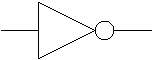
\includegraphics[height=0.75cm]{fig/non.pdf} & 
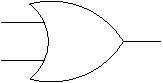
\includegraphics[height=0.75cm]{fig/ou.pdf}  &
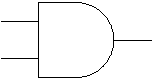
\includegraphics[height=0.75cm]{fig/et.pdf}  \\
\hline
 & \tt not (a or b) & \tt not (a and b) \\
 & 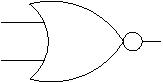
\includegraphics[height=0.75cm]{fig/nonOu.pdf} & \includegraphics[height=0.75cm]{fig/nonEt.pdf}\\
\hline
\end{tabular}
\hfill
\begin{tabular}{ll}
\multicolumn{2}{l}{$\forall a, b, c \in \{0;1\}$ :}\\
\makebox[0.5cm]{} & {$a + 0 = a$} \hspace*{5mm} {$a \cdot 1 = a$}\\
 & {$a + 1 = 1$} \hspace*{5mm} {$a \cdot 0 = 0$}\\
 & {$a + a = a$} \hspace*{5mm} {$a \cdot a = a$}\\
 & {$a + \overline{a} = 1$} \hspace*{5mm} {$a \cdot \overline{a} = 0$}\\
 & {$a + (a \cdot b) = a$} \hspace*{5mm} {$a \cdot (a + b) = a$}\\
 & {$\overline{\overline{a}}  = a$} \hspace*{5mm} $\overline{a + b} = \overline{a} \cdot \overline{b}$ \hspace*{5mm} $\overline{a\cdot b} = \overline{a} + \overline{b}$\\
 & {$(a+b) = (b+a)$} \hspace*{5mm}  {$(a \cdot b) = (b \cdot a)$} \\
 & {$(a+b)+c = a+(b+c)$} \\ 
 & {$(a\cdot b)\cdot c = a\cdot (b\cdot c)$} \\
 & {$a + (b \cdot c) = (a+b) \cdot (a+c)$} \\ 
 & {$a \cdot (b+ c) = (a \cdot b)+(a\cdot c)$} 
\end{tabular}$$
\caption{Opérateurs logiques en \python}
\label{table:python:operateurs-logiques}
\end{table}

%-------------------------------------------------------------------------
\subsection{Alternative simple}\label{tests:cours:alternative-simple}
%-------------------------------------------------------------------------

L'instruction « {\tt if} \ldots\ {\tt else} » teste une condition. 
Si la condition
est vraie, alors le bloc d'instructions {\tt blocIf} après le « {\tt :} » est exécuté.
Si la condition est fausse, c'est le bloc d'instructions {\tt blocElse} après le « {\tt else:} » 
(sinon) qui est exécuté. Seul l'un des 2 blocs est donc exécuté.

\begin{definition}[alternative simple]
L'alternative simple est une instruction de contrôle du flux d'instructions 
qui permet de choisir entre deux instructions selon qu'une condition est vérifiée ou non.
\end{definition}

La figure \ref{figure:uml:alternative-simple} montre
qu'une alternative se comporte comme un aiguillage de chemin de fer 
dans le flux d'instructions. 
Un « {\tt if ... else} » ouvre  deux voies correspondant à deux traitements différents, 
et seule une de ces voies sera empruntée (un seul des deux traitements est
exécuté). 
A ce titre, le test simple de la section \ref{tests:cours:test-simple} précédente est équivalent 
à une alternative simple où on explicite le fait de ne rien faire (instruction {\tt pass})
dans le bloc d'instructions associé au {\tt else}.

\begin{figure}[ht]
$$\begin{minipage}{10cm}
\begin{Verbatim}
if condition : blocIf
else         : blocElse
\end{Verbatim}
\end{minipage}$$
$${\includegraphics[width=10cm]{fig/uml1.pdf}}$$
$$\begin{minipage}{10cm}
L'étiquette {\tt [condition]} signifie qu'on passe par la voie correspondante 
si la condition est vérifiée ({\tt True}), sinon on passe par la voie étiquettée
{\tt [else]}.
\end{minipage}$$
\caption{Alternative simple en \python}
\label{figure:uml:alternative-simple}
\end{figure}

Mais il y a des situations où deux voies ne suffisent pas : on utilise
alors des alternatives simples en cascade (ou alternatives multiples). 

%-------------------------------------------------------------------------
\subsection{Alternative multiple}\label{tests:cours:alternative-multiple}
%-------------------------------------------------------------------------

L'instruction « {\tt if} \ldots\ {\tt elif} » teste une première condition. 
Si cette condition est vraie, alors le bloc d'instructions {\tt blocIf} 
est exécuté. Si la première condition est fausse, on teste la deuxième ({\tt condition1}).
Si la deuxième condition est vérifiée, c'est le bloc d'instructions {\tt blocElif1} après le premier « {\tt elif:} » 
(sinon-si) qui est exécuté; sinon on teste la condition suivante ({\tt condition2}).
Si elle est vérifiée, c'est le bloc d'instructions {\tt blocElif2} après le deuxième « {\tt elif:} » 
qui est exécuté et ainsi de suite. Si aucune des conditions n'est vérifiée, c'est le bloc d'instructions
{\tt blocElse} qui est exécuté. Dans tous les cas, un seul des blocs est donc exécuté.

\begin{definition}[alternative multiple]
L'alternative multiple est une instruction de contrôle du flux d'instructions 
qui permet de choisir entre plusieurs instructions en cascadant des alternatives simples.
\end{definition}

%-------------------------------------------------------------------------
\section{Vie courante : mention au baccalauréat}\label{tests:vie-courante}
%-------------------------------------------------------------------------

\subsection{Objectif}\label{tests:vie-courante:objectif}
\begin{description}
\item[Principal : ] mettre en \oe uvre l'instruction d'alternative multiple.
\item[Secondaire :] déterminer la mention au bac.
\end{description}

\subsection{Syntaxe \python}\label{tests:vie-courante:python}
\noindent\begin{minipage}[t]{0.3\textwidth}
test simple\footnotesize
\begin{Verbatim}
if condition : bloc
\end{Verbatim}
\end{minipage}
\hfill
\begin{minipage}[t]{0.3\textwidth}
alternative simple\footnotesize
\begin{Verbatim}
if condition : bloc1
else         : bloc2
\end{Verbatim}
\end{minipage}
\hfill
\begin{minipage}[t]{0.3\textwidth}
alternative multiple\footnotesize
\begin{Verbatim}
if   condition1 : bloc1
elif condition2 : bloc2
elif condition3 : bloc3
...
else            : blocn
\end{Verbatim}
\end{minipage}

\subsection{Enoncé}\label{tests:vie-courante:enonce}

\subsection{Méthode}\label{tests:vie-courante:methode}

\subsection{Résultat}\label{tests:vie-courante:resultat}

\subsection{Vérification}\label{tests:vie-courante:verification}

\subsection{Généricité}\label{tests:vie-courante:genericite}

\subsection{Entraînement}\label{tests:vie-courante:entrainement}

%-------------------------------------------------------------------------
\section{Jeux : 421}
%-------------------------------------------------------------------------

\subsection{Objectif}\label{tests:jeux:objectif}
\begin{description}
\item[Principal : ] mettre en \oe uvre l'instruction d'alternative multiple.
\item[Secondaire :] .
\end{description}

\subsection{Syntaxe \python}\label{tests:jeux:python}
\noindent\begin{minipage}[t]{0.3\textwidth}
test simple\footnotesize
\begin{Verbatim}
if condition : bloc
\end{Verbatim}
\end{minipage}
\hfill
\begin{minipage}[t]{0.3\textwidth}
alternative simple\footnotesize
\begin{Verbatim}
if condition : bloc1
else         : bloc2
\end{Verbatim}
\end{minipage}
\hfill
\begin{minipage}[t]{0.3\textwidth}
alternative multiple\footnotesize
\begin{Verbatim}
if   condition1 : bloc1
elif condition2 : bloc2
elif condition3 : bloc3
...
else            : blocn
\end{Verbatim}
\end{minipage}

\subsection{Enoncé}\label{tests:jeux:enonce}

\subsection{Méthode}\label{tests:jeux:methode}

\subsection{Résultat}\label{tests:jeux:resultat}

\subsection{Vérification}\label{tests:jeux:verification}

\subsection{Généricité}\label{tests:jeux:genericite}

\subsection{Entraînement}\label{tests:jeux:entrainement}


%-------------------------------------------------------------------------
\section{Textes : }
%-------------------------------------------------------------------------

\subsection{Objectif}\label{tests:textes:objectif}
Mettre en \oe uvre l'instruction d'alternative multiple sur un exemple de type « textes ».

\subsection{Syntaxe \python}\label{tests:textes:python}
\noindent\begin{minipage}[t]{0.3\textwidth}
test simple\footnotesize
\begin{Verbatim}
if condition : bloc
\end{Verbatim}
\end{minipage}
\hfill
\begin{minipage}[t]{0.3\textwidth}
alternative simple\footnotesize
\begin{Verbatim}
if condition : bloc1
else         : bloc2
\end{Verbatim}
\end{minipage}
\hfill
\begin{minipage}[t]{0.3\textwidth}
alternative multiple\footnotesize
\begin{Verbatim}
if   condition1 : bloc1
elif condition2 : bloc2
elif condition3 : bloc3
...
else            : blocn
\end{Verbatim}
\end{minipage}

\subsection{Enoncé}\label{tests:textes:enonce}

\subsection{Méthode}\label{tests:textes:methode}

\subsection{Résultat}\label{tests:textes:resultat}

\subsection{Vérification}\label{tests:textes:verification}

\subsection{Généricité}\label{tests:textes:genericite}

\subsection{Entraînement}\label{tests:textes:entrainement}

%-------------------------------------------------------------------------
\section{Nombres : }
%-------------------------------------------------------------------------

\subsection{Objectif}\label{tests:nombres:objectif}
\begin{description}
\item[Principal : ] mettre en \oe uvre l'instruction d'alternative multiple.
\item[Secondaire :] .
\end{description}

\subsection{Syntaxe \python}\label{tests:nombres:python}
\noindent\begin{minipage}[t]{0.3\textwidth}
test simple\footnotesize
\begin{Verbatim}
if condition : bloc
\end{Verbatim}
\end{minipage}
\hfill
\begin{minipage}[t]{0.3\textwidth}
alternative simple\footnotesize
\begin{Verbatim}
if condition : bloc1
else         : bloc2
\end{Verbatim}
\end{minipage}
\hfill
\begin{minipage}[t]{0.3\textwidth}
alternative multiple\footnotesize
\begin{Verbatim}
if   condition1 : bloc1
elif condition2 : bloc2
elif condition3 : bloc3
...
else            : blocn
\end{Verbatim}
\end{minipage}

\subsection{Enoncé}\label{tests:nombres:enonce}

\subsection{Méthode}\label{tests:nombres:methode}

\subsection{Résultat}\label{tests:nombres:resultat}

\subsection{Vérification}\label{tests:nombres:verification}

\subsection{Généricité}\label{tests:nombres:genericite}

\subsection{Entraînement}\label{tests:nombres:entrainement}

%-------------------------------------------------------------------------
\section{Figures : }
%-------------------------------------------------------------------------

\subsection{Objectif}\label{tests:figures:objectif}
\begin{description}
\item[Principal : ] mettre en \oe uvre l'instruction d'alternative multiple.
\item[Secondaire :] .
\end{description}

\subsection{Syntaxe \python}\label{tests:figures:python}
\noindent\begin{minipage}[t]{0.3\textwidth}
test simple\footnotesize
\begin{Verbatim}
if condition : bloc
\end{Verbatim}
\end{minipage}
\hfill
\begin{minipage}[t]{0.3\textwidth}
alternative simple\footnotesize
\begin{Verbatim}
if condition : bloc1
else         : bloc2
\end{Verbatim}
\end{minipage}
\hfill
\begin{minipage}[t]{0.3\textwidth}
alternative multiple\footnotesize
\begin{Verbatim}
if   condition1 : bloc1
elif condition2 : bloc2
elif condition3 : bloc3
...
else            : blocn
\end{Verbatim}
\end{minipage}

\subsection{Enoncé}\label{tests:figures:enonce}

\subsection{Méthode}\label{tests:figures:methode}

\subsection{Résultat}\label{tests:figures:resultat}

\subsection{Vérification}\label{tests:figures:verification}

\subsection{Généricité}\label{tests:figures:genericite}

\subsection{Entraînement}\label{tests:figures:entrainement}

%-------------------------------------------------------------------------
\section{Mathématiques : graphe de fonction}
%-------------------------------------------------------------------------

\subsection{Objectif}\label{tests:maths:objectif}
\begin{description}
\item[Principal : ] mettre en \oe uvre l'instruction d'alternative multiple.
\item[Secondaire :] .
\end{description}

\subsection{Syntaxe \python}\label{tests:maths:python}
\noindent\begin{minipage}[t]{0.3\textwidth}
test simple\footnotesize
\begin{Verbatim}
if condition : bloc
\end{Verbatim}
\end{minipage}
\hfill
\begin{minipage}[t]{0.3\textwidth}
alternative simple\footnotesize
\begin{Verbatim}
if condition : bloc1
else         : bloc2
\end{Verbatim}
\end{minipage}
\hfill
\begin{minipage}[t]{0.3\textwidth}
alternative multiple\footnotesize
\begin{Verbatim}
if   condition1 : bloc1
elif condition2 : bloc2
elif condition3 : bloc3
...
else            : blocn
\end{Verbatim}
\end{minipage}

\subsection{Enoncé}\label{tests:maths:enonce}
On considère dans $\mathbb{R}$ la fonction continue $f$, affine par morceaux,  
définie sur $[-5;5]$  par le graphe ci-dessous et $\forall x < -5, f(x) = f(-5)$
et $\forall x > 5, f(x) = f(5)$. 
$$%\begin{minipage}{6.75cm}
\begin{tikzpicture}[scale=0.5]\footnotesize
\draw[color=lightgray](-5,-2) grid[xstep=1,ystep=1] (5,2);
\foreach \x in {-5,-4,...,5} \draw(\x,-2) node[below]{\x};
\foreach \y in {-2,-1,...,2} \draw(-5,\y) node[left]{\y};
\filldraw(0,0) circle (0.1);
\draw[->] (-5,0) -- (5,0);
\draw (5,0) node[right]{$x$} ;
\draw[->] (0,-2) -- (0,2);
\draw (0,2) node[above]{$y$};
\draw[color=blue] (-5,1) -- (-4,1) -- (-3,0) -- (-2,1) -- (0,-2) -- (1,2) -- (4,-1) -- (5,1);
%\draw (-4.5,1) node[above]{\Pisymbol{pzd}{172}};
%\draw (-3.5,0.5) node[above]{\Pisymbol{pzd}{173}};
%\draw (-2.5,0.5) node[below]{\Pisymbol{pzd}{174}};
%\draw (-1,-0.5) node[below]{\Pisymbol{pzd}{175}};
%\draw (0.5,0) node[right]{\Pisymbol{pzd}{176}};
%\draw (2.5,0.5) node[right]{\Pisymbol{pzd}{177}};
%\draw (4.5,0) node[above]{\Pisymbol{pzd}{178}};
\end{tikzpicture}
%\end{minipage}
$$
Proposer une instruction de type « alternative multiple » qui permettra de calculer 
la fonction $y = f(x)$ $\forall x \in \mathbb{R}$.

\subsection{Méthode}\label{tests:maths:methode}
Il s'agit de déterminer la valeur $y = f(x)$ d'une fonction continue affine par morceaux sur $\mathbb{R}$. L'axe des réels $]-\infty,x_1,x_2,\ldots,x_n,+\infty[$ est donc vu comme une
succession d'intervalles $]-\infty,x_1[$, $[x_1,x_2[$, \ldots, $[x_{n-1},x_n[$ et
$[x_n,+\infty[$ sur lesquels la fonction $f$ est définie respectivement par les fonctions $f_1$, $f_2$, \ldots, $f_n$ et $f_{n+1}$ :
$$\begin{tabular}{l@{ $=$ }l@{ $\forall x \in$ }l}
$y = f(x)$ 	& $f_1(x)$		& $]-\infty,x_1[$ \\
			& $f_2(x)$ 		& $[x_1,x_2[$ \\
			& $f_3(x)$ 		& $[x_2,x_3[$ \\
			& \multicolumn{2}{l}{\ldots} \\
			& $f_n(x)$ 		& $[x_{n-1},x_n[$\\
			& $f_{n+1}(x)$ 	& $[x_n,+\infty[$
\end{tabular}$$
Chacune des fonctions $f_i$ correspond à une droite d'équation $y = a_ix+b_i$ où $a_i$
représente la pente de la droite et $b_i$ son ordonnée à l'origine.
Lorsqu'on connaît 2 points $M(x_M,y_M)$ et $N(x_N,y_N)$ 
d'une droite d'équation $y = ax + b$, les coefficients $a$ (pente de la droite) 
et $b$ (ordonnée à l'origine) de la droite sont obtenus
par résolution du système de 2 équations : $y_M =ax_M + b$ et $y_N = ax_N + b$. 
On obtient alors $a$ et $b$ :

$$\begin{minipage}{6.75cm}
\begin{tikzpicture}[scale=0.5]\footnotesize
\draw[color=lightgray](-5,-2) grid[xstep=1,ystep=1] (5,2);
\foreach \x in {-5,-4,...,5} \draw(\x,-2) node[below]{\x};
\foreach \y in {-2,-1,...,2} \draw(-5,\y) node[left]{\y};
\filldraw(0,0) circle (0.1);
\filldraw(-1,-1) circle (0.1);
\draw (-1,-1) node[below]{$M$};
\draw(-1,0) node[above]{$x_M$};
\draw(0,-1) node[right]{$y_M$};
\draw (-1,-1) -- (-1,0);
\draw (-1,-1) -- (0,-1);
\filldraw(2,1) circle (0.1);
\draw (2,1) node[above]{$N$};
\draw(2,0) node[below]{$x_N$};
\draw(0,1) node[left]{$y_N$};
\draw (2,1) -- (2,0);
\draw (2,1) -- (0,1);
\draw[->] (-5,0) -- (5,0);
\draw (5,0) node[right]{$x$} ;
\draw[->] (0,-2) -- (0,2);
\draw (0,2) node[above]{$y$};
\draw[color=blue] (-4,-3) -- (5,3);
\draw[color=blue](4.3,2.3) node[above,rotate=33.69]{$y = ax + b$};
\end{tikzpicture}
\end{minipage}
\hfill
\begin{minipage}{8.75cm}
$$\displaystyle a = \frac{y_N - y_M}{x_N - x_M} \mbox{ et } \displaystyle b = \frac{y_Mx_N - y_Nx_M}{x_N - x_M}$$
Pour la droite ci-contre :
$$\displaystyle 
a = \frac{1 - (-1)}{2 - (-1)} = \frac{2}{3} \mbox{ et } \displaystyle 
b = \frac{(-1)\cdot 2 - 1\cdot(-1)}{2 - (-1)} = -\frac{1}{3}
$$
On vérifie graphiquement ces résultats : pour passer de $M$ à $N$, on
se déplace de $\Delta x = 3$ horizontalement puis de $\Delta y = 2$ verticalement 
(d'où la pente $a = \Delta y/\Delta x = 2/3$),
et la droite coupe bien l'axe des ordonnées en $y = -1/3$.
\end{minipage}$$
Une fois déterminés les coefficients $a_i$ et $b_i$ de chaque droite, on détermine
la valeur de la fonction $y = f(x)$ par une alternative multiple du genre :
$$\begin{minipage}{5.5cm}\tt
if   x < $x_1$ : y = $a_1$*x + $b_1$\\
elif x < $x_2$ : y = $a_2$*x + $b_2$\\
elif x < $x_3$ : y = $a_3$*x + $b_3$\\
...\\
elif x < $x_n$ : y = $a_n$*x + $b_n$\\
else           : y = $a_{n+1}$*x + $b_{n+1}$
\end{minipage}$$

\subsection{Résultat}\label{tests:maths:resultat}
On applique la méthode précédente à la fonction $f$ de l'énoncé.
Il faut donc déterminer les équations de droite 
correspondant aux différents segments du graphe de la fonction, à savoir :
$$\begin{minipage}{9cm}
\begin{tikzpicture}[scale=0.5]\footnotesize
\draw[color=lightgray](-5,-2) grid[xstep=1,ystep=1] (5,2);
\foreach \x in {-5,-4,...,5} \draw(\x,-2) node[below]{\x};
\foreach \y in {-2,-1,...,2} \draw(-5,\y) node[left]{\y};
\filldraw(0,0) circle (0.1);
\draw[->] (-5,0) -- (5,0);
\draw (5,0) node[right]{$x$} ;
\draw[->] (0,-2) -- (0,2);
\draw (0,2) node[above]{$y$};
\draw[color=blue] (-5,1) -- (-4,1) -- (-3,0) -- (-2,1) -- (0,-2) -- (1,2) -- (4,-1) -- (5,1);
\draw (-4.5,1) node[above]{\Pisymbol{pzd}{172}};
\draw (-3.5,0.5) node[above]{\Pisymbol{pzd}{173}};
\draw (-2.5,0.5) node[below]{\Pisymbol{pzd}{174}};
\draw (-1,-0.5) node[below]{\Pisymbol{pzd}{175}};
\draw (0.5,0) node[right]{\Pisymbol{pzd}{176}};
\draw (2.5,0.5) node[right]{\Pisymbol{pzd}{177}};
\draw (4.5,0) node[above]{\Pisymbol{pzd}{178}};
\end{tikzpicture}
\end{minipage}
\hfill
\begin{minipage}{3cm}
\begin{itemize}
\item[\Pisymbol{pzd}{172}] $y = 1$
\item[\Pisymbol{pzd}{173}] $y = -x -3$
\item[\Pisymbol{pzd}{174}] $y = x + 3$
\item[\Pisymbol{pzd}{175}] $y = -3x/2 - 2$
\item[\Pisymbol{pzd}{176}] $y = 4x - 2$
\item[\Pisymbol{pzd}{177}] $y = -x + 3$
\item[\Pisymbol{pzd}{178}] $y = 2x - 9$
\end{itemize}
\end{minipage}$$

\noindent\begin{minipage}[t]{7cm}
Compte-tenu de ces équations, le code ci-contre
permet de calculer $y = f(x)$, y compris pour $x < -5$ ($y = f(-5) =1$) et 
$x > 5$ ($y = f(5) = 1$).

Remarque : on aurait pu simplifier les deux premières lignes de ce code en\\
\centerline{\texttt{if x < -4 : y = 1}}
car les instructions associées sont iden\-tiques (ie. les fonctions
affines sont identiques sur $]-\infty,-5[$ et $[-5,-4[$).
\end{minipage}
\hfill
\begin{minipage}[t]{8cm}\footnotesize
\begin{lstlisting}[caption=\textbf{graphe d'une fonction}]
if   x < -5 : y = 1
elif x < -4 : y = 1
elif x < -3 : y = -x - 3
elif x < -2 : y = x + 3
elif x <  0 : y = -3*x/2 - 2
elif x <  1 : y = 4*x - 2
elif x <  4 : y = -x + 3
elif x <  5 : y = 2*x - 9
else        : y = 1
\end{lstlisting}
\end{minipage}

\subsection{Vérification}\label{tests:maths:verification}
Pour tester le résultat précédent, 
on peut comparer les valeurs obtenues par le calcul avec celles lues
directement sur le graphe pour quelques points caractéristiques.
Ces points de mesure sont choisis judicieusement : ils ne correspondent 
pas aux bornes des intervalles déjà prises en compte dans la méthode
mais plutôt à des points où la fonction s'annule 
(exemples : $x = -4/3$, $1/2$, $3$ ou $9/2$)
ou à des points d'abscisses aux n\oe uds de la grille de lecture 
(exemples : $x = -1$ ou $x = 2$).
On peut vérifier par exemple pour $x = -1$ 
($y = f(-1) = -1/2$) et $x = 3$ ($y = f(3) = 0$).
$$\begin{minipage}{7.5cm}\footnotesize
\begin{Verbatim}
>>> x = -1
>>> if x < -4 : y = 1
elif   x < -3 : y = -x - 3
elif   x < -2 : y = x + 3
elif   x <  0 : y = -3*x/2 - 2
elif   x <  1 : y = 4*x - 2
elif   x <  4 : y = -x + 3
elif   x <  5 : y = 2*x - 9
else          : y = 1

>>> y
-0.5
\end{Verbatim}
\end{minipage}
\hfill
\begin{minipage}{7.5cm}\footnotesize
\begin{Verbatim}
>>> x = 3
>>> if x < -4 : y = 1
elif   x < -3 : y = -x - 3
elif   x < -2 : y = x + 3
elif   x <  0 : y = -3*x/2 - 2
elif   x <  1 : y = 4*x - 2
elif   x <  4 : y = -x + 3
elif   x <  5 : y = 2*x - 9
else          : y = 1

>>> y
0
\end{Verbatim}
\end{minipage}$$
On obtient bien par le calcul les résultats lus sur la grille.

\subsection{Généricité}\label{tests:maths:genericite}
Pour vérifier la généricité de la méthode précédente,
proposer une alternative multiple pour chacune des 2 fonctions définies sur $[-5;5]$ 
par les graphes ci-dessous et $\forall x <~-5, f(x) = f(-5)$
et $\forall x > 5, f(x) = f(5)$.

\begin{minipage}{7cm}
\begin{enumerate}
\item 
\begin{tikzpicture}[scale=0.5]\footnotesize
\draw[color=lightgray](-5,-2) grid[xstep=1,ystep=1] (5,2);
\foreach \x in {-5,-4,...,5} \draw(\x,-2) node[below]{\x};
\foreach \y in {-2,-1,...,2} \draw(-5,\y) node[left]{\y};
\filldraw(0,0) circle (0.1);
\draw[->] (-5,0) -- (5,0); 
\draw (5,0) node[right]{$x$} ;
\draw[->] (0,-2) -- (0,2);
\draw (0,2) node[above]{$y$};
\draw[color=blue] (-5,0) -- (-4,-1) -- (-3,1) -- (1,-2) -- (2,-2) -- (5,-1);
\end{tikzpicture}
\end{enumerate}
\end{minipage}
\hfill
\begin{minipage}{7cm}
\begin{enumerate}\setcounter{enumi}{1}
\item 
\begin{tikzpicture}[scale=0.5]\footnotesize
\draw[color=lightgray](-5,-2) grid[xstep=1,ystep=1] (5,2);
\foreach \x in {-5,-4,...,5} \draw(\x,-2) node[below]{\x};
\foreach \y in {-2,-1,...,2} \draw(-5,\y) node[left]{\y};
\filldraw(0,0) circle (0.1);
\draw[->] (-5,0) -- (5,0);
\draw (5,0) node[right]{$x$} ;
\draw[->] (0,-2) -- (0,2);
\draw (0,2) node[above]{$y$};
\draw[color=blue] (-5,-1) -- (-4,-1) -- (-4,0) -- (-2,2) -- (0,2) -- (1,-1) -- (1,-1) -- (3,1) -- (3,-1) -- (5,-1);
\end{tikzpicture}
\end{enumerate}
\end{minipage}

\subsection{Entraînement}\label{tests:maths:entrainement}
Utiliser une alternative multiple pour déterminer les racines réelles
d'un trinôme du second degré $ax^2 + bx + c$ à coefficients $a$, $b$ et $c$ réels.


%-------------------------------------------------------------------------
\section{Physique : états de l'eau}
%-------------------------------------------------------------------------

\subsection{Objectif}\label{tests:physique:objectif}
\begin{description}
\item[Principal : ] mettre en \oe uvre l'instruction d'alternative multiple.
\item[Secondaire :] .
\end{description}

\subsection{Syntaxe \python}\label{tests:physique:python}

\subsection{Enoncé}\label{tests:physique:enonce}


\subsection{Méthode}\label{tests:physique:methode}

\subsection{Résultat}\label{tests:physique:resultat}

\subsection{Vérification}\label{tests:physique:verification}

\subsection{Généricité}\label{tests:physique:genericite}

\subsection{Entraînement}\label{tests:physique:entrainement}

%-------------------------------------------------------------------------
\section{Informatique : }
%-------------------------------------------------------------------------

\subsection{Objectif}\label{tests:informatique:objectif}
\begin{description}
\item[Principal : ] mettre en \oe uvre l'instruction d'alternative multiple.
\item[Secondaire :] .
\end{description}

\subsection{Syntaxe \python}\label{tests:informatique:python}
\noindent\begin{minipage}[t]{0.3\textwidth}
test simple\footnotesize
\begin{Verbatim}
if condition : bloc
\end{Verbatim}
\end{minipage}
\hfill
\begin{minipage}[t]{0.3\textwidth}
alternative simple\footnotesize
\begin{Verbatim}
if condition : bloc1
else         : bloc2
\end{Verbatim}
\end{minipage}
\hfill
\begin{minipage}[t]{0.3\textwidth}
alternative multiple\footnotesize
\begin{Verbatim}
if   condition1 : bloc1
elif condition2 : bloc2
elif condition3 : bloc3
...
else            : blocn
\end{Verbatim}
\end{minipage}

\subsection{Enoncé}\label{tests:informatique:enonce}

\subsection{Méthode}\label{tests:informatique:methode}

\subsection{Résultat}\label{tests:informatique:resultat}

\subsection{Vérification}\label{tests:informatique:verification}

\subsection{Généricité}\label{tests:informatique:genericite}

\subsection{Entraînement}\label{tests:informatique:entrainement}

%-------------------------------------------------------------------------
\section{Retours d'expériences}\label{tests:retours}
%-------------------------------------------------------------------------

%-------------------------------------------------------------------------
\subsection{Méthode}\label{tests:retours:methode}

%-------------------------------------------------------------------------
\subsection{Résultat}\label{tests:retours:resultat}

%-------------------------------------------------------------------------
\subsection{Vérification}\label{tests:retours:verification}


%
\chapter{Boucles}\label{instructions:boucles}
	% mrv-boucles.tex

%-------------------------------------------------------------------------
\section{Rappels de cours}\label{boucles:cours}
%-------------------------------------------------------------------------
\begin{enumerate}
\item Comment éviter de répéter explicitement plusieurs fois de suite la même 
	séquence d'instructions ? 
\item Comment éviter de savoir à l'avance combien de fois il faut répéter
	la séquence pour obtenir le bon résultat ? 
\end{enumerate}

De nouvelles instructions de contrôle de flux sont introduites pour répondre
à ces questions : les instructions itératives. 
On parle également de boucles, de répétitions ou encore d'itérations.
Nous distinguerons 2 variantes d'instructions itératives (Table \ref{table:python:boucles}):
l'itération conditionnelle (\texttt{while}) et le parcours de séquences (\texttt{for}).
\begin{table}[ht]
$$\begin{tabular}{|l|l|}
\hline
\multicolumn{2}{|c|}{Instructions itératives}\\
\hline
itération conditionnelle & {\begin{minipage}[t]{6cm}\tt while condition : blocWhile \\ \mbox{} \end{minipage}} \\
\hline
parcours de séquence & {\begin{minipage}[t]{7cm}\tt for element in sequence : blocFor \\ \mbox{} \end{minipage}} \\
\hline
\multicolumn{2}{p{10cm}}{où {\tt while}, {\tt for} et {\tt in} sont des mots réservés, 
{\tt condition} une expression booléenne (à valeur {\tt True} ou {\tt False}), 
{\tt element} un élément de la séquence {\tt sequence}
et {\tt bloc...} un bloc d'instructions.}
\end{tabular}$$
\caption{Instructions itératives en \python}
\label{table:python:boucles}
\end{table}

A propos des instructions itératives,
on parle souvent des boucles « {\tt while} » ou des boucles « {\tt for} » 
dans le jargon des informaticiens.

%-------------------------------------------------------------------------
\subsection{Itération conditionnelle}
%-------------------------------------------------------------------------
%$$\includegraphics[width=7.5cm]{fig/uml4.pdf}$$

L'instruction « {\tt while} » permet de répéter plusieurs fois une même instruction 
(Figure \ref{figure:uml:while}) : le bloc d'instructions {\tt blocWhile} est exécuté 
tant que (\emph{while}) la condition est vérifiée. On arrête dès que la condition est fausse; 
on dit alors qu'on « sort » de la boucle. 

On commence par tester la condition; si elle
est vérifiée, on exécute le bloc d'instructions {\tt blocWhile} 
(encore appelé le «~corps~» de la boucle) puis on reteste la condition : 
la condition est ainsi évaluée avant chaque exécution du corps 
de la boucle; si la condition est à nouveau vérifiée on réexécute le bloc 
d'instructions {\tt blocWhile} (on dit qu'on « repasse » dans la boucle)
et ainsi de suite jusqu'à ce que la condition devienne fausse, 
auquel cas on « sort » de la boucle.

\begin{definition}[itération conditionnelle]
L'itération conditionnelle est une instruction de contrôle du flux d'instructions
qui permet sous condition préalable de répéter zéro ou plusieurs fois la même instruction.
\end{definition}

Dans une itération conditionnelle, la condition doit évoluer au cours des différents passages
dans la boucle afin de pouvoir sortir de la boucle. 
En ce qui concerne le nombre de passages dans la boucle, deux cas extrèmes peuvent se produire : 
\begin{itemize}
\item la condition n'est pas vérifiée la première fois : 
	on ne passe alors jamais dans la boucle.
	
	Exemple : 
	\begin{minipage}[t]{5cm}
	\begin{Verbatim}
	x = 4
	y = 0
	while x < 0 : y = y + x
	\end{Verbatim}
	\end{minipage}\hfill
	\begin{minipage}[t]{7.5cm}\footnotesize
	$x$ est positif; la condition $x < 0$ n'est donc pas vérifiée la première
	fois : on ne rentre pas dans la boucle.
	\end{minipage}
\item la condition n'est jamais fausse : on ne sort jamais de la boucle; 
	on dit qu'on a affaire à une boucle « sans fin ».

	Exemple : 
	\begin{minipage}[t]{5cm}
	\begin{Verbatim}
	x = 4
	y = 0
	while y >= 0 : y = y + x
	\end{Verbatim}
	\end{minipage}\hfill
	\begin{minipage}[t]{7.5cm}\footnotesize
	$y$ est initialement nul : on rentre dans la boucle;
	l'instruction du corps de la boucle ne peut qu'incrémenter $y$
	puisque $x$ est positif : $y$ sera donc toujours positif et on 
	ne sortira jamais de la boucle.
	\end{minipage}
\end{itemize}
Le cas de la boucle « sans fin » est évidemment dû le plus souvent à une erreur involontaire
qu'il faut savoir détecter assez vite pour éviter un programme qui « tourne » indéfiniment
sans s'arrêter.

Dans tous les cas, que l'on connaisse ou non {\em a priori} le nombre de passages dans la boucle, on peut
toujours utiliser l'itération conditionnelle (boucle {\tt while}) pour répéter plusieurs fois un bloc
d'instructions à condition de connaître la condition d'arrêt pour sortir de la boucle.
\begin{itemize}
\item Lorsqu'on connaît {\em a priori} le nombre de passages dans la boucle, 
	il suffit de définir un compteur qui compte le nombre
	de fois où on passe dans la boucle.
	On initialise correctement ce compteur avant la boucle, 
	on incrémente le compteur dans le corps de la boucle
	et on sort de la boucle lorsque ce compteur dépasse le nombre de fois connu
	où on doit passer dans la boucle.
\item Lorsqu'on ne connaît pas {\em a priori} le nombre de passages dans la boucle, 
	il faut absolument déterminer la condition d'arrêt
	de l'algorithme.
	Il faut également s'assurer que cette condition sera bien atteinte au bout d'un certain 
	nombre de passages dans la boucle.
\end{itemize}


%-------------------------------------------------------------------------
\subsection{Parcours de séquences}
%-------------------------------------------------------------------------
Il est fréquent de manipuler des suites ordonnées d'éléments comme 
les chaînes de caractères (exemple : {\tt s = "123"}), les tableaux
(exemple : {\tt t = [1,2,3]}) et les n-uplets (exemple : {\tt u = 1,2,3}).
Chaque élément d'une séquence est accessible par son rang dans la séquence 
grâce à l'opérateur « crochets » : {\tt sequence[rang]} (exemples : {\tt s[1]}, {\tt t[2]} ou {\tt u[0]}) et par convention, 
le premier élément d'une séquence a le rang {\tt 0} (exemples : {\tt s[1]} est le $2^{\grave eme}$
élément de la chaîne {\tt s}, {\tt t[2]} le $3^{\grave eme}$ élément du tableau {\tt t}
et {\tt u[0]} le $1^{er}$ élément du n-uplet {\tt u}).

\begin{minipage}[t]{4cm}
\begin{Verbatim}
>>> s = "123"
>>> s[1]
'2'
\end{Verbatim}
\end{minipage}
\hfill
\begin{minipage}[t]{4cm}
\begin{Verbatim}
>>> t = [1,2,3]
>>> t[2]
3
\end{Verbatim}
\end{minipage}
\hfill
\begin{minipage}[t]{4cm}
\begin{Verbatim}
>>> u = 1,2,3
>>> u[0]
1
\end{Verbatim}
\end{minipage}

\begin{definition}[séquence]
Une séquence est une suite ordonnée d'éléments, éventuellement vide, 
accessibles par leur rang dans la séquence.
\end{definition}

\noindent Les principales opérations sur les séquences sont listées 
dans le tableau ci-dessous
$$\begin{tabular}{|l|p{9cm}|}
\hline 
\makebox[5.5cm][l]{\bf Operation} &	\bf Result 	\\
\hline
\tt x in s      & {\tt True} if an item of {\tt s} is equal to {\tt x}, else {\tt False} \\ 	
\tt x not in s 	& {\tt False} if an item of {\tt s} is equal to {\tt x}, else {\tt True}\\
\hline 	
\tt s1 + s2 	& the concatenation of {\tt s1} and {\tt s2}\\ 	 
\tt s * n, n*s 	& {\tt n} copies of {\tt s} concatenated \\	
\hline
\hline
\tt s[i] 	& {\tt i}'th item of {\tt s}, origin {\tt 0}\\ 	
\tt s[i: j]     & \\
\tt s[i: j:step]& Slice of {\tt s} from {\tt i} (included) to {\tt j}(excluded). 
                  Optional {\tt step} value, possibly negative (default: {\tt 1}). \\	
\hline
\tt len(s) 	& Length of s \\	 
\tt min(s) 	& Smallest item of s \\	
\tt max(s) 	& Largest item of s \\
\hline
\hline
\tt range([start,] end [, step]) & Returns list of ints from {\tt >=} {\tt start} and {\tt <} {\tt end}.\newline
	With 1 arg, list from {\tt 0..arg-1}\newline
	With 2 args, list from {\tt start..end-1}\newline
	With 3 args, list from {\tt start} up to {\tt end} by {\tt step}\\
\hline
\end{tabular}$$

La dernière fonction de ce tableau crée un tableau d'entiers compris entre {\tt start} inclus
(= 0 par défaut) et {\tt end} exclus par pas de {\tt step} (= 1 par défaut).

\begin{minipage}[t]{5cm}
\begin{Verbatim}
>>> range(3)
[0, 1, 2]
>>> range(3,9,2)
[3, 5, 7]
>>> range(7,0,-1)
[7, 6, 5, 4, 3, 2, 1]
\end{Verbatim}
\end{minipage}
\hfill
\begin{minipage}[t]{5cm}
\begin{Verbatim}
>>> s = "bonjour"
>>> range(len(s))
[0, 1, 2, 3, 4, 5, 6]
>>> t = [4,2,6,5,3]
>>> range(max(t),min(t),-1)
[6, 5, 4, 3]
\end{Verbatim}
\end{minipage}
\hfill
\begin{minipage}[t]{5cm}
\begin{Verbatim}
>>> u1 = 10,12,14
>>> u2 = 'a','b','c'
>>> range(len(u1+u2))
[0, 1, 2, 3, 4, 5]
>>> range(len(2*u2[0:2]))
[0, 1, 2, 3]
\end{Verbatim}
\end{minipage}
\vspace*{1mm}

\noindent Il existe une instruction de contrôle adaptée au parcours de séquence :
$$\fbox{\tt for element in sequence : blocFor}$$
$$\begin{minipage}{6.5cm}équivalente à : 
\begin{minipage}[t]{4cm}
\begin{Verbatim}
i = 0
while i < len(s):
    element = sequence[i]
    blocFor
    i = i + 1
\end{Verbatim}
\end{minipage}
\end{minipage}$$

%-------------------------------------------------------------------------
\subsection{Imbrications de boucles}
%-------------------------------------------------------------------------
De la même manière que l'on peut cascader des alternatives simples
(voir section \ref{sub:alternatives}), on peut encapsuler une boucle 
dans une autre boucle.


Les instructions composées ont toujours la même structure : 
une ligne d'en-tête terminée par un double point ({:}), suivie
d'une ou de plusieurs instructions indentées (décalées à droite)
sous cette ligne d'en-tête (figure \ref{fig:bloc}).

\begin{minipage}[t]{5cm}
\begin{Verbatim}
ligne d'en-tête:
    première instruction du bloc
    ...
    dernière instruction du bloc
\end{Verbatim}
\end{minipage}

\noindent S'il y a plusieurs instructions indentées sous la ligne d'en-tête, elles doivent l'être exactement au
même niveau (décalage de 4 caractères espace, par exemple). Ces instructions indentées
constituent ce qu'on appellera désormais un bloc d'instructions. Un bloc d'instructions est une
suite d'instructions formant un ensemble logique, qui n'est exécuté que dans certaines conditions
définies dans la ligne d'en-tête. Dans l'exemple précédent, les deux lignes
d'instructions indentées sous la ligne contenant l'instruction « {\tt while i < 10:} » constituent un même 
bloc logique : ces deux lignes ne sont exécutées -- toutes les deux -- que si la condition testée 
avec l'instruction {\tt while} est vérifiée, c'est-à-dire si le multiplicateur {\tt i}
est tel que {\tt 1 <= i < 10}.


%-------------------------------------------------------------------------
\subsection{Exécutions de boucles}
%-------------------------------------------------------------------------
La maîtrise de l'algorithmique requiert deux qualités complémentaires \cite{darmengeat} :
\begin{itemize}
\item il faut avoir une certaine intuition, car aucun algorithme ne permet de 
	savoir {\em a priori} quelles instructions permettront d'obtenir le résultat 
	recherché. C'est là qu'intervient la forme « d'intelligence » 
	requise pour l'algorithmique : la « créativité » de l'informaticien. 
	Il y a des gens qui possèdent au 
	départ davantage cette intuition que les autres.  
	Cependant, les réflexes, cela s'acquiert (en particulier, l'annexe \ref{invariant}
	page \pageref{invariant} présente une méthode pour aider à construire des boucles). 
	Et ce qu'on appelle l'intuition n'est finalement que de l'expérience accumulée,
	tellement répétée que le raisonnement, au départ laborieux, finit par 
	devenir «~spontané~».
\item il faut être méthodique et rigoureux. En effet, chaque fois qu'on écrit 
	une série d'instructions que l'on croit justes, il faut systématiquement 
	se mettre mentalement à la place de la machine qui va les exécuter
	(sur papier ou dans sa tête) afin de vérifier si le résultat obtenu 
	est bien celui que l'on voulait. 
	Cette opération ne requiert pas d'intuition. Mais elle reste néanmoins indispensable
	si l'on ne veut pas écrire des algorithmes à l'« aveuglette ».
	Et petit à petit, à force de pratique, on fera
	de plus en plus souvent l'économie de cette dernière étape : 
	l'expérience fera qu'on « verra » le résultat produit par les instructions, 
	au fur et à mesure qu'on les écrira. 
	Naturellement, cet apprentissage est long, et demande des heures de 
	travail patient. 
	Aussi, dans un premier temps, il faut éviter de sauter les étapes : la vérification méthodique, 
	pas à pas, de chacun des algorithmes représente plus de la moitié du travail à accomplir\ldots
	et le gage de progrès.
\end{itemize}

Pour améliorer la compréhension d'une boucle, on peut « tracer » son exécution de tête,
à la main ou par programme. Dans tous les cas, l'idée est de suivre pas à pas
l'évolution des variables qui interviennent dans la boucle : on détermine leur valeur 
juste avant la boucle, à la fin de chaque itération et juste après la boucle.

%-------------------------------------------------------------------------
\subsection{Construction d'une boucle}
%-------------------------------------------------------------------------
Un algorithme est un mécanisme qui fait passer un « système » d'une « situation »
dite initiale (ou précondition) à une « situation » finale (postcondition ou but). 
Le couple (situation initiale, situation finale) est appelé spécification de l'algorithme. 
L'algorithmique vise donc à construire rationnellement des algorithmes à partir de 
leur spécification.

Le raisonnement qui permet de passer d'une compréhension intuitive d'un
tel énoncé à l'algorithme n'est pas toujours facile à concevoir d'un coup. 
Dans le cas d'une boucle on pourra systématiser la conception de l'algorithme
autour de 4 étapes (d'après \cite{didier} et \cite{guyomard}):
\begin{enumerate}
\item {\bf Invariant} (ou hypothèse de récurrence) : « Le clou est planté dans la planche ».
\item {\bf Condition d'arrêt} : « La tête touche la planche ».
\item {\bf Progression} : « Frapper un coup de marteau de façon à enfoncer un peu plus le clou ».
\item {\bf Initialisation} : « Planter légèrement le clou à la main ».
\end{enumerate}
Il faut noter que les étapes 1 et 2 définissent des situations
tandis que les étapes 3 et 4 concernent des actions. 
Dans cette section, on notera les situations entre crochets ({\tt []}) pour les distinguer
des actions.
\begin{itemize}
\item La recherche d'un invariant est l'étape clé autour de laquelle s'articule la conception des boucles. 
	La conjonction de l'invariant et de la condition d'arrêt conduit logiquement au but recherché :
	$$\fbox{\begin{minipage}{13cm}\tt
	[« invariant » and « condition d'arrêt »] $\Rightarrow$ [« postcondition »]
	\end{minipage}}$$
	La condition d'arrêt seule n'implique pas le but.

\item La progression doit :
	\begin{itemize}
	\item conserver l'invariant.
		Plus précisément, la progression est un fragment d'algorithme
		défini par les situations initiale et finale suivantes :\\
		\mbox{}\hspace*{5mm}situation initiale : {\tt [« invariant » and not « condition d'arrêt »]}\\
		\mbox{}\hspace*{5mm}situation finale : {\tt [« invariant »]}\\ 
		$$\fbox{\begin{minipage}{13cm}\tt
		\mbox{}[« invariant » and not « condition d'arrêt »]\\
		\mbox{}« progression »\\
		\mbox{}[« invariant »]
		\end{minipage}}$$
	\item faire effectivement progresser vers le but pour faire en sorte que la condition 
		d'arrêt soit atteinte au bout d'un temps fini.
	\end{itemize}
\item  L'initialisation doit instaurer l'invariant. 
	Plus précisément, elle doit, partant de la précondi\-tion, atteindre l'invariant.
		$$\fbox{\begin{minipage}{13cm}\tt
		\mbox{}[« précondition »]\\
		\mbox{}« initialisation »\\
		\mbox{}[« invariant »]
		\end{minipage}}$$

\end{itemize}
D'une manière plus générale, les 4 étapes de construction d'une boucle
sont les suivantes :
\begin{enumerate}
\item {\bf Invariant :} proposer une situation générale décrivant le problème posé (hypothèse de
	récurrence). C'est cette étape qui est la plus délicate car elle exige de faire 
	preuve d'imagination.

\item {\bf Condition d'arrêt :} à partir de la situation générale imaginée en [1], on doit
	formuler la condition qui permet d'affirmer que l'algorithme a terminé son travail. 
	La situation dans laquelle il se trouve alors est appelée situation finale.
	La condition d'arrêt fait sortir de la boucle.

\item {\bf Progression :} se « rapprocher » de la situation finale, tout en faisant le nécessaire pour
	conserver à chaque étape une situation générale analogue à celle retenue en [1].
	La progression conserve l'invariant.
	
\item {\bf Initialisation :} initialiser les variables introduites dans l'invariant 
	pour que celui-ci soit vérifié avant d'entrer dans la boucle.
	L'initialisation « instaure » l'invariant.
	
\item {\bf Boucle finale :} Une fois les 4 étapes précédentes menées à leur terme, l'algorithme recherché 
	aura la structure finale suivante (figure \ref{fig:invariant}) :
	$$\begin{minipage}[t]{4cm}
	\begin{verbatim}
	[« précondition »]
	« initialisation »
	[« invariant »]
	while not [« condition d'arrêt »] :
	    « progression »
	    [« invariant »]
	[« postcondition »]
	\end{verbatim}
	\end{minipage}$$
	Quand on sort de la boucle, la situation finale attendue est atteinte.
	
	Dans la pratique, on ne garde que les instructions :
	$$\fbox{\begin{minipage}[t]{8cm}\tt
	« initialisation »\\
	while [not « condition d'arrêt »] : \\
	\mbox{}\ \ \ \ « progression »
	\end{minipage}}$$
	\begin{minipage}[t]{6cm}
	Exemple de la puissance \ref{ex:puissance} :\\
	{\tt k = 1}\\
	{\tt p = x}\\
	{\tt while not k > n: }\\
	{\tt \mbox{}\ \ \ \ p = p*x}\\
	{\tt \mbox{}\ \ \ \ k = k + 1}
	\end{minipage}
	\hfill
	\begin{minipage}[t]{6cm}
	Exemple du pgcd \ref{ex:pgcd3} :\\
	{\tt while not b == 0:}\\
	{\tt \mbox{}\ \ \ \ r = a\%b}\\
	{\tt \mbox{}\ \ \ \ a = b}\\
	{\tt \mbox{}\ \ \ \ b = r}
	\end{minipage}
	
	Un des problèmes, pour l'apprenti informaticien, est que la boucle finale
	ainsi obtenue ne fait pas apparaître explicitement l'invariant dans le code. 
	L'invariant est une aide conceptuelle pour construire la boucle, 
	mais pas pour l'exécuter.
\end{enumerate}

\begin{definition}
Un invariant de boucle est une propriété vérifiée tout au long de 
l'exécution de la boucle. 
\end{definition}

Cette façon de procéder permet de « prouver » la validité de l'algorithme au fur et à
mesure de son élaboration. En effet la situation générale choisie en [1] est en fait l'invariant 
qui caractérise la boucle {\tt while}.
Cette situation est satisfaite au départ grâce à l'initialisation de l'étape [4]; 
elle reste vraie à chaque itération (étape [3]). Ainsi lorsque la condition d'arrêt (étape [2])
est atteinte cette situation nous permet d'affirmer que le problème est résolu.
C'est également en analysant l'étape [3] qu'on peut prouver la terminaison de l'algorithme.


%-------------------------------------------------------------------------
\section{Vie courante : }\label{boucles:vie-courante}
%-------------------------------------------------------------------------

\subsection{Objectif}\label{boucles:vie-courante:objectif}
\begin{description}
\item[Principal : ] mettre en \oe uvre une instruction d'itération.
\item[Secondaire :] .
\end{description}


\subsection{Syntaxe \python}\label{boucles:vie-courante:python}

\subsection{Enoncé}\label{boucles:vie-courante:enonce}

\subsection{Méthode}\label{boucles:vie-courante:methode}

\subsection{Résultat}\label{boucles:vie-courante:resultat}

\subsection{Vérification}\label{boucles:vie-courante:verification}

\subsection{Généricité}\label{boucles:vie-courante:genericite}

\subsection{Entraînement}\label{boucles:vie-courante:entrainement}

%-------------------------------------------------------------------------
\section{Jeux : }\label{boucles:jeux}
%-------------------------------------------------------------------------

\subsection{Objectif}\label{boucles:jeux:objectif}
\begin{description}
\item[Principal : ] mettre en \oe uvre une instruction d'itération.
\item[Secondaire :] .
\end{description}

\subsection{Syntaxe \python}\label{boucles:jeux:python}

\subsection{Enoncé}\label{boucles:jeux:enonce}

\subsection{Méthode}\label{boucles:jeux:methode}

\subsection{Résultat}\label{boucles:jeux:resultat}

\subsection{Vérification}\label{boucles:jeux:verification}

\subsection{Généricité}\label{boucles:jeux:genericite}

\subsection{Entraînement}\label{boucles:jeux:entrainement}


%-------------------------------------------------------------------------
\section{Textes : compter les voyelles}\label{boucles:textes}
%-------------------------------------------------------------------------

\subsection{Objectif}\label{boucles:textes:objectif}
\begin{description}
\item[Principal : ] mettre en \oe uvre une instruction d'itération.
\item[Secondaire :] compter le nombre de voyelles dans une chaîne de caractères.
\end{description}

\subsection{Syntaxe \python}\label{boucles:textes:python}

\subsection{Enoncé}\label{boucles:textes:enonce}

\subsection{Méthode}\label{boucles:textes:methode}

\subsection{Résultat}\label{boucles:textes:resultat}

\subsection{Vérification}\label{boucles:textes:verification}

\subsection{Généricité}\label{boucles:textes:genericite}

\subsection{Entraînement}\label{boucles:textes:entrainement}

%-------------------------------------------------------------------------
\section{Nombres : conversion décimal $\rightarrow$ binaire}\label{boucles:nombres}
%-------------------------------------------------------------------------

\subsection{Objectif}\label{boucles:nombres:objectif}
\begin{description}
\item[Principal : ] mettre en \oe uvre une instruction d'itération.
\item[Secondaire :] convertir un entier décimal en un entier binaire.
\end{description}

\subsection{Syntaxe \python}\label{boucles:nombres:python}

\subsection{Enoncé}\label{boucles:nombres:enonce}

\subsection{Méthode}\label{boucles:nombres:methode}

\subsection{Résultat}\label{boucles:nombres:resultat}

\subsection{Vérification}\label{boucles:nombres:verification}

\subsection{Généricité}\label{boucles:nombres:genericite}

\subsection{Entraînement}\label{boucles:nombres:entrainement}

%-------------------------------------------------------------------------
\section{Figures : tracé d'un heptagone régulier}\label{boucles:figures}
%-------------------------------------------------------------------------

\subsection{Objectif}\label{boucles:figures:objectif}
\begin{description}
\item[Principal : ] mettre en \oe uvre une instruction d'itération.
\item[Secondaire :] tracer un heptagone régulier.
\end{description}

\subsection{Syntaxe \python}\label{boucles:figures:python}

\subsection{Enoncé}\label{boucles:figures:enonce}

\subsection{Méthode}\label{boucles:figures:methode}

\subsection{Résultat}\label{boucles:figures:resultat}

\subsection{Vérification}\label{boucles:figures:verification}

\subsection{Généricité}\label{boucles:figures:genericite}

\subsection{Entraînement}\label{boucles:figures:entrainement}

%-------------------------------------------------------------------------
\section{Mathématiques : intégration de $\cos(x)$}\label{boucles:maths}
%-------------------------------------------------------------------------

\subsection{Objectif}\label{boucles:maths:objectif}
\begin{description}
\item[Principal : ] mettre en \oe uvre une instruction d'itération.
\item[Secondaire :] calculer l'intégrale de la fonction cosinus.
\end{description}

\subsection{Syntaxe \python}\label{boucles:maths:python}

\subsection{Enoncé}\label{boucles:maths:enonce}

\subsection{Méthode}\label{boucles:maths:methode}

\subsection{Résultat}\label{boucles:maths:resultat}

\subsection{Vérification}\label{boucles:maths:verification}

\subsection{Généricité}\label{boucles:maths:genericite}

\subsection{Entraînement}\label{boucles:maths:entrainement}

%-------------------------------------------------------------------------
\section{Physique : sorties d'un circuit logique}\label{boucles:physique}
%-------------------------------------------------------------------------

\subsection{Objectif}\label{boucles:physique:objectif}
\begin{description}
\item[Principal : ] mettre en \oe uvre une instruction d'itération.
\item[Secondaire :] déterminer la table de vérité d'un circuit logique.
\end{description}

\subsection{Syntaxe \python}\label{boucles:physique:python}

\subsection{Enoncé}\label{boucles:physique:enonce}

\subsection{Méthode}\label{boucles:physique:methode}

\subsection{Résultat}\label{boucles:physique:resultat}

\subsection{Vérification}\label{boucles:physique:verification}

\subsection{Généricité}\label{boucles:physique:genericite}

\subsection{Entraînement}\label{boucles:physique:entrainement}

%-------------------------------------------------------------------------
\section{Informatique : }\label{boucles:informatique}
%-------------------------------------------------------------------------

\subsection{Objectif}\label{boucles:informatique:objectif}
\begin{description}
\item[Principal : ] mettre en \oe uvre l'instruction d'itération.
\item[Secondaire :] .
\end{description}

\subsection{Syntaxe \python}\label{boucles:informatique:python}

\subsection{Enoncé}\label{boucles:informatique:enonce}

\subsection{Méthode}\label{boucles:informatique:methode}

\subsection{Résultat}\label{boucles:informatique:resultat}

\subsection{Vérification}\label{boucles:informatique:verification}

\subsection{Généricité}\label{boucles:informatique:genericite}

\subsection{Entraînement}\label{boucles:informatique:entrainement}


%-------------------------------------------------------------------------
\section{Retours d'expériences}\label{boucles:retours}
%-------------------------------------------------------------------------

%-------------------------------------------------------------------------
\subsection{Méthode}\label{boucles:retours:methode}

%-------------------------------------------------------------------------
\subsection{Résultat}\label{boucles:retours:resultat}

%-------------------------------------------------------------------------
\subsection{Vérification}\label{boucles:retours:verification}


%
\chapter{Instructions imbriquées}\label{instructions:imbrication}
	% mrv-instructions.tex

%-------------------------------------------------------------------------
\section{Rappels de cours}\label{instructions:cours}
%-------------------------------------------------------------------------

%-------------------------------------------------------------------------
\section{Vie courante}\label{instructions:vie-courante}
%-------------------------------------------------------------------------
\begin{description}
\item[Principal : ] mettre en \oe uvre les instructions de base : affectation, tests, boucles.
\item[Secondaire :] .
\end{description}

\subsection{Objectif}\label{instructions:vie-courante:objectif}

\subsection{Syntaxe \python}\label{instructions:vie-courante:python}

\subsection{Enoncé}\label{instructions:vie-courante:enonce}

\subsection{Méthode}\label{instructions:vie-courante:methode}

\subsection{Résultat}\label{instructions:vie-courante:resultat}

\subsection{Vérification}\label{instructions:vie-courante:verification}

\subsection{Généricité}\label{instructions:vie-courante:genericite}

\subsection{Entraînement}\label{instructions:vie-courante:entrainement}

%-------------------------------------------------------------------------
\section{Jeux : drapeau tricolore}\label{instructions:jeux}
%-------------------------------------------------------------------------

\subsection{Objectif}\label{instructions:jeux:objectif}
\begin{description}
\item[Principal : ] mettre en \oe uvre les instructions de base : affectation, tests, boucles.
\item[Secondaire :] .
\end{description}


\subsection{Syntaxe \python}\label{instructions:jeux:python}

\subsection{Enoncé}\label{instructions:jeux:enonce}

\subsection{Méthode}\label{instructions:jeux:methode}

\subsection{Résultat}\label{instructions:jeux:resultat}

\subsection{Vérification}\label{instructions:jeux:verification}

\subsection{Généricité}\label{instructions:jeux:genericite}

\subsection{Entraînement}\label{instructions:jeux:entrainement}


%-------------------------------------------------------------------------
\section{Textes : recherche d'un motif}\label{instructions:textes}
%-------------------------------------------------------------------------

\subsection{Objectif}\label{instructions:textes:objectif}
\begin{description}
\item[Principal : ] mettre en \oe uvre les instructions de base : affectation, tests, boucles.
\item[Secondaire :] recherche une chaîne de caractères au sein d'une autre chaîne.
\end{description}


\subsection{Syntaxe \python}\label{instructions:textes:python}

\subsection{Enoncé}\label{instructions:textes:enonce}

\subsection{Méthode}\label{instructions:textes:methode}

\subsection{Résultat}\label{instructions:textes:resultat}

\subsection{Vérification}\label{instructions:textes:verification}

\subsection{Généricité}\label{instructions:textes:genericite}

\subsection{Entraînement}\label{instructions:textes:entrainement}

%-------------------------------------------------------------------------
\section{Nombres : crible d'Eratostène}\label{instructions:nombres}
%-------------------------------------------------------------------------

\subsection{Objectif}\label{instructions:nombres:objectif}
\begin{description}
\item[Principal : ] mettre en \oe uvre les instructions de base : affectation, tests, boucles.
\item[Secondaire :] déterminer les $n$ premiers nombres premiers.
\end{description}


\subsection{Syntaxe \python}\label{instructions:nombres:python}

\subsection{Enoncé}\label{instructions:nombres:enonce}

\subsection{Méthode}\label{instructions:nombres:methode}

\subsection{Résultat}\label{instructions:nombres:resultat}

\subsection{Vérification}\label{instructions:nombres:verification}

\subsection{Généricité}\label{instructions:nombres:genericite}

\subsection{Entraînement}\label{instructions:nombres:entrainement}

%-------------------------------------------------------------------------
\section{Figures : }\label{instructions:figures}
%-------------------------------------------------------------------------

\subsection{Objectif}\label{instructions:figures:objectif}
\begin{description}
\item[Principal : ] mettre en \oe uvre les instructions de base : affectation, tests, boucles.
\item[Secondaire :] .
\end{description}


\subsection{Syntaxe \python}\label{instructions:figures:python}

\subsection{Enoncé}\label{instructions:figures:enonce}

\subsection{Méthode}\label{instructions:figures:methode}

\subsection{Résultat}\label{instructions:figures:resultat}

\subsection{Vérification}\label{instructions:figures:verification}

\subsection{Généricité}\label{instructions:figures:genericite}

\subsection{Entraînement}\label{instructions:figures:entrainement}

%-------------------------------------------------------------------------
\section{Mathématiques : zéro d'une fonction}\label{instructions:maths}
%-------------------------------------------------------------------------

\subsection{Objectif}\label{instructions:maths:objectif}
\begin{description}
\item[Principal : ] mettre en \oe uvre les instructions de base : affectation, tests, boucles.
\item[Secondaire :] .
\end{description}


\subsection{Syntaxe \python}\label{instructions:maths:python}

\subsection{Enoncé}\label{instructions:maths:enonce}

\subsection{Méthode}\label{instructions:maths:methode}

\subsection{Résultat}\label{instructions:maths:resultat}

\subsection{Vérification}\label{instructions:maths:verification}

\subsection{Généricité}\label{instructions:maths:genericite}

\subsection{Entraînement}\label{instructions:maths:entrainement}

%-------------------------------------------------------------------------
\section{Physique : }\label{instructions:physique}
%-------------------------------------------------------------------------

\subsection{Objectif}\label{instructions:physique:objectif}
\begin{description}
\item[Principal : ] mettre en \oe uvre les instructions de base : affectation, tests, boucles.
\item[Secondaire :] .
\end{description}


\subsection{Syntaxe \python}\label{instructions:physique:python}

\subsection{Enoncé}\label{instructions:physique:enonce}

\subsection{Méthode}\label{instructions:physique:methode}

\subsection{Résultat}\label{instructions:physique:resultat}

\subsection{Vérification}\label{instructions:physique:verification}

\subsection{Généricité}\label{instructions:physique:genericite}

\subsection{Entraînement}\label{instructions:physique:entrainement}

%-------------------------------------------------------------------------
\section{Informatique : }\label{instructions:informatique}
%-------------------------------------------------------------------------

\subsection{Objectif}\label{instructions:informatique:objectif}
\begin{description}
\item[Principal : ] mettre en \oe uvre les instructions de base : affectation, tests, boucles.
\item[Secondaire :] .
\end{description}


\subsection{Syntaxe \python}\label{instructions:informatique:python}

\subsection{Enoncé}\label{instructions:informatique:enonce}

\subsection{Méthode}\label{instructions:informatique:methode}

\subsection{Résultat}\label{instructions:informatique:resultat}

\subsection{Vérification}\label{instructions:informatique:verification}

\subsection{Généricité}\label{instructions:informatique:genericite}

\subsection{Entraînement}\label{instructions:informatique:entrainement}


%-------------------------------------------------------------------------
\section{Retours d'expériences}\label{instructions:retours}
%-------------------------------------------------------------------------

%-------------------------------------------------------------------------
\subsection{Algorithmes}\label{instructions:retours:algorithmes}

%-------------------------------------------------------------------------
\subsection{\mrv : méthode}\label{instructions:retours:methode}

%-------------------------------------------------------------------------
\subsection{\mrv : résultat}\label{instructions:retours:resultat}

%-------------------------------------------------------------------------
\subsection{\mrv : vérification}\label{instructions:retours:verification}

%
%
%%-------------------------------------------------------------------------
\part{Fonctions}\label{fonctions}
%
\chapter{Spécification}\label{fonctions:specification}
%	\input{mrv-specification.tex}
%
\chapter{Appels de fonctions}\label{fonctions:appels}
%	\input{mrv-appels.tex}
%
\chapter{Récursivité}\label{fonctions:recursivite}
%	\input{mrv-recursivite.tex}
%
%
%%-------------------------------------------------------------------------
\part{Tout en un}\label{tout-en-un}
%
\chapter{Vie courante : recherche d'un chemin}\label{tout-en-un:vie-courante}
%
\chapter{Jeux : }\label{tout-en-un:jeux}
%	http://norvig.com/sudoku.html
%
\chapter{Textes : cryptographie}\label{tout-en-un:textes}
%
\chapter{Nombres : calculateur en base b}\label{tout-en-un:nombres}
%
\chapter{Figures : construction de figures}\label{tout-en-un:figures}
%
\chapter{Mathématiques : systèmes linéaires}\label{tout-en-un:maths}
%
\chapter{Physique : équation différentielle}\label{tout-en-un:physique}
%
\chapter{Informatique : machine de Turing}\label{tout-en-un:informatique}
%



%-------------------------------------------------------------------------
\end{document}
%-------------------------------------------------------------------------
